\section{Годограф Найквиста}
Рассмотрим передаточную функцию физически реализуемой разомкнутой системы вида: 
\begin{equation}
    W_o(s) = \frac{s^5 + b_4s^4 + b_3s^3 + b_2s^2 + b_1s + b_0}{s^5 + a_4s^4 + a_3s^3 + a_2s^2 + a_1s + a_0}
    \label{task1:object}
\end{equation}
и передаточную функцию замкнутой системы:
\begin{equation}
    W_c(s) = \frac{s^5 + b_4s^4 + b_3s^3 + b_2s^2 + b_1s + b_0}{2s^5 + (a_4 + b_4)s^4 + (a_3 + b_3)s^3 + (a_2 + b_2)s^2 + (a_1 + b_1)s + (a_0 + b_0)}
\end{equation}
исходя из того, что все полюса объекта вещественные, можно переписать \ref{task1:object} в виде:
\begin{equation}
    W_o(s) = \frac{(s - z_1)(s - z_2)(s - z_3)(s - z_4)(s - z_5)}{(s - p_1)(s - p_2)(s - p_3)(s - p_4)(s - p_5)}
\end{equation}
Перепишем передаточную функцию замкнутой системы в виде:
\begin{equation}
    W_c(s) = \frac{(s - z_1)(s - z_2)(s - z_3)(s - z_4)(s - z_5)}{2(s - k_1)(s - k_2)(s - k_3)(s - k_4)(s - k_5)}
\end{equation}

Введем функцию $C(Z):R^5\rightarrow R^5$, аргумент которой -- вектор корней полинома пятой степени, а значение -- вектор коэффициентов соответствующего полинома. Тогда можно записать:
\begin{equation}
    C(Z) = \begin{bmatrix}
        -z_1z_2z_3z_4z_5 \\ 
        -z_1 - z_2 - z_3 - z_4 - z_5 \\
        z_1z_2 + z_1z_3 + z_1z_4 + z_1z_5 + z_2z_3 + z_2z_4 + z_2z_5 + z_3z_4 + z_3z_5 + z_4z_5 \\
        -z_1z_2z_3 - z_1z_2z_4 - z_1z_2z_5 - z_1z_3z_4 - z_1z_3z_5 - z_1z_4z_5 - z_2z_3z_4 - z_2z_3z_5 - z_2z_4z_5 - z_3z_4z_5 \\
        z_1z_2z_3z_4 + z_1z_2z_3z_5 + z_1z_2z_4z_5 + z_1z_3z_4z_5 + z_2z_3z_4z_5 \\
    \end{bmatrix}
    \notag
\end{equation}

Задавшись полюсами $P$ разомкнутой системы и полюсами $K$ замкнутой системы, найдем передаточные
функции замкнутой и разомкнутой системы:
\begin{equation}
    A = C(P) \quad B = C(K) - A 
\end{equation}
где 
\begin{equation}
    A = \begin{bmatrix}
         a_0 \\ a_1 \\ a_2 \\ a_3 \\ a_4
    \end{bmatrix} \quad 
    B = \begin{bmatrix}
        b_0 \\ b_1 \\ b_2 \\ b_3 \\ b_4
    \end{bmatrix}
\end{equation}


\subsection{Система 1}
Зададимся системой с полюсами $P$:
\begin{equation}
    P = \begin{bmatrix}
        1 & 1.5 & 2 & -1 & -2
    \end{bmatrix}
\end{equation}
И полюсами замкнутой системы $K$:
\begin{equation}
    K = \begin{bmatrix}
        1 & 1.5 & -2.5 & -1 & -2
    \end{bmatrix}
\end{equation}

% a_4 = -1.500000, a_3 = -5.000000, a_2 = 7.500000, a_1 = 4.000000, a_0 = -6.000000
% b_4 = 4.500000, b_3 = 2.250000, b_2 = -18.000000, b_1 = -2.250000, b_0 = 13.500000
Запишем передаточные функции разомкнутой и замкнутой системы:
\begin{equation}
    W_{\text{o}} = \frac{s^5 +4.50s^4 +2.25s^3 -18.00s^2 -2.25s +13.50}{s^5 -1.50s^4 -5.00s^3 +7.50s^2 +4.00s -6.00}
\end{equation}
\begin{equation}
    W_{\text{c}} = \frac{s^5 +4.50s^4 +2.25s^3 -18.00s^2 -2.25s +13.50}{2s^5 +3.00s^4 -2.75s^3 -10.50s^2 +1.75s +7.50}
\end{equation}

Карты расположения полюсов передаточных функций приведены на рисунках \ref{fig:task1_poles:open} и \ref{fig:task1_poles:closed} соответственно.
% 2 figures on the same line
\begin{figure}[ht!]
    \centering
    \begin{subfigure}{0.5\textwidth}
        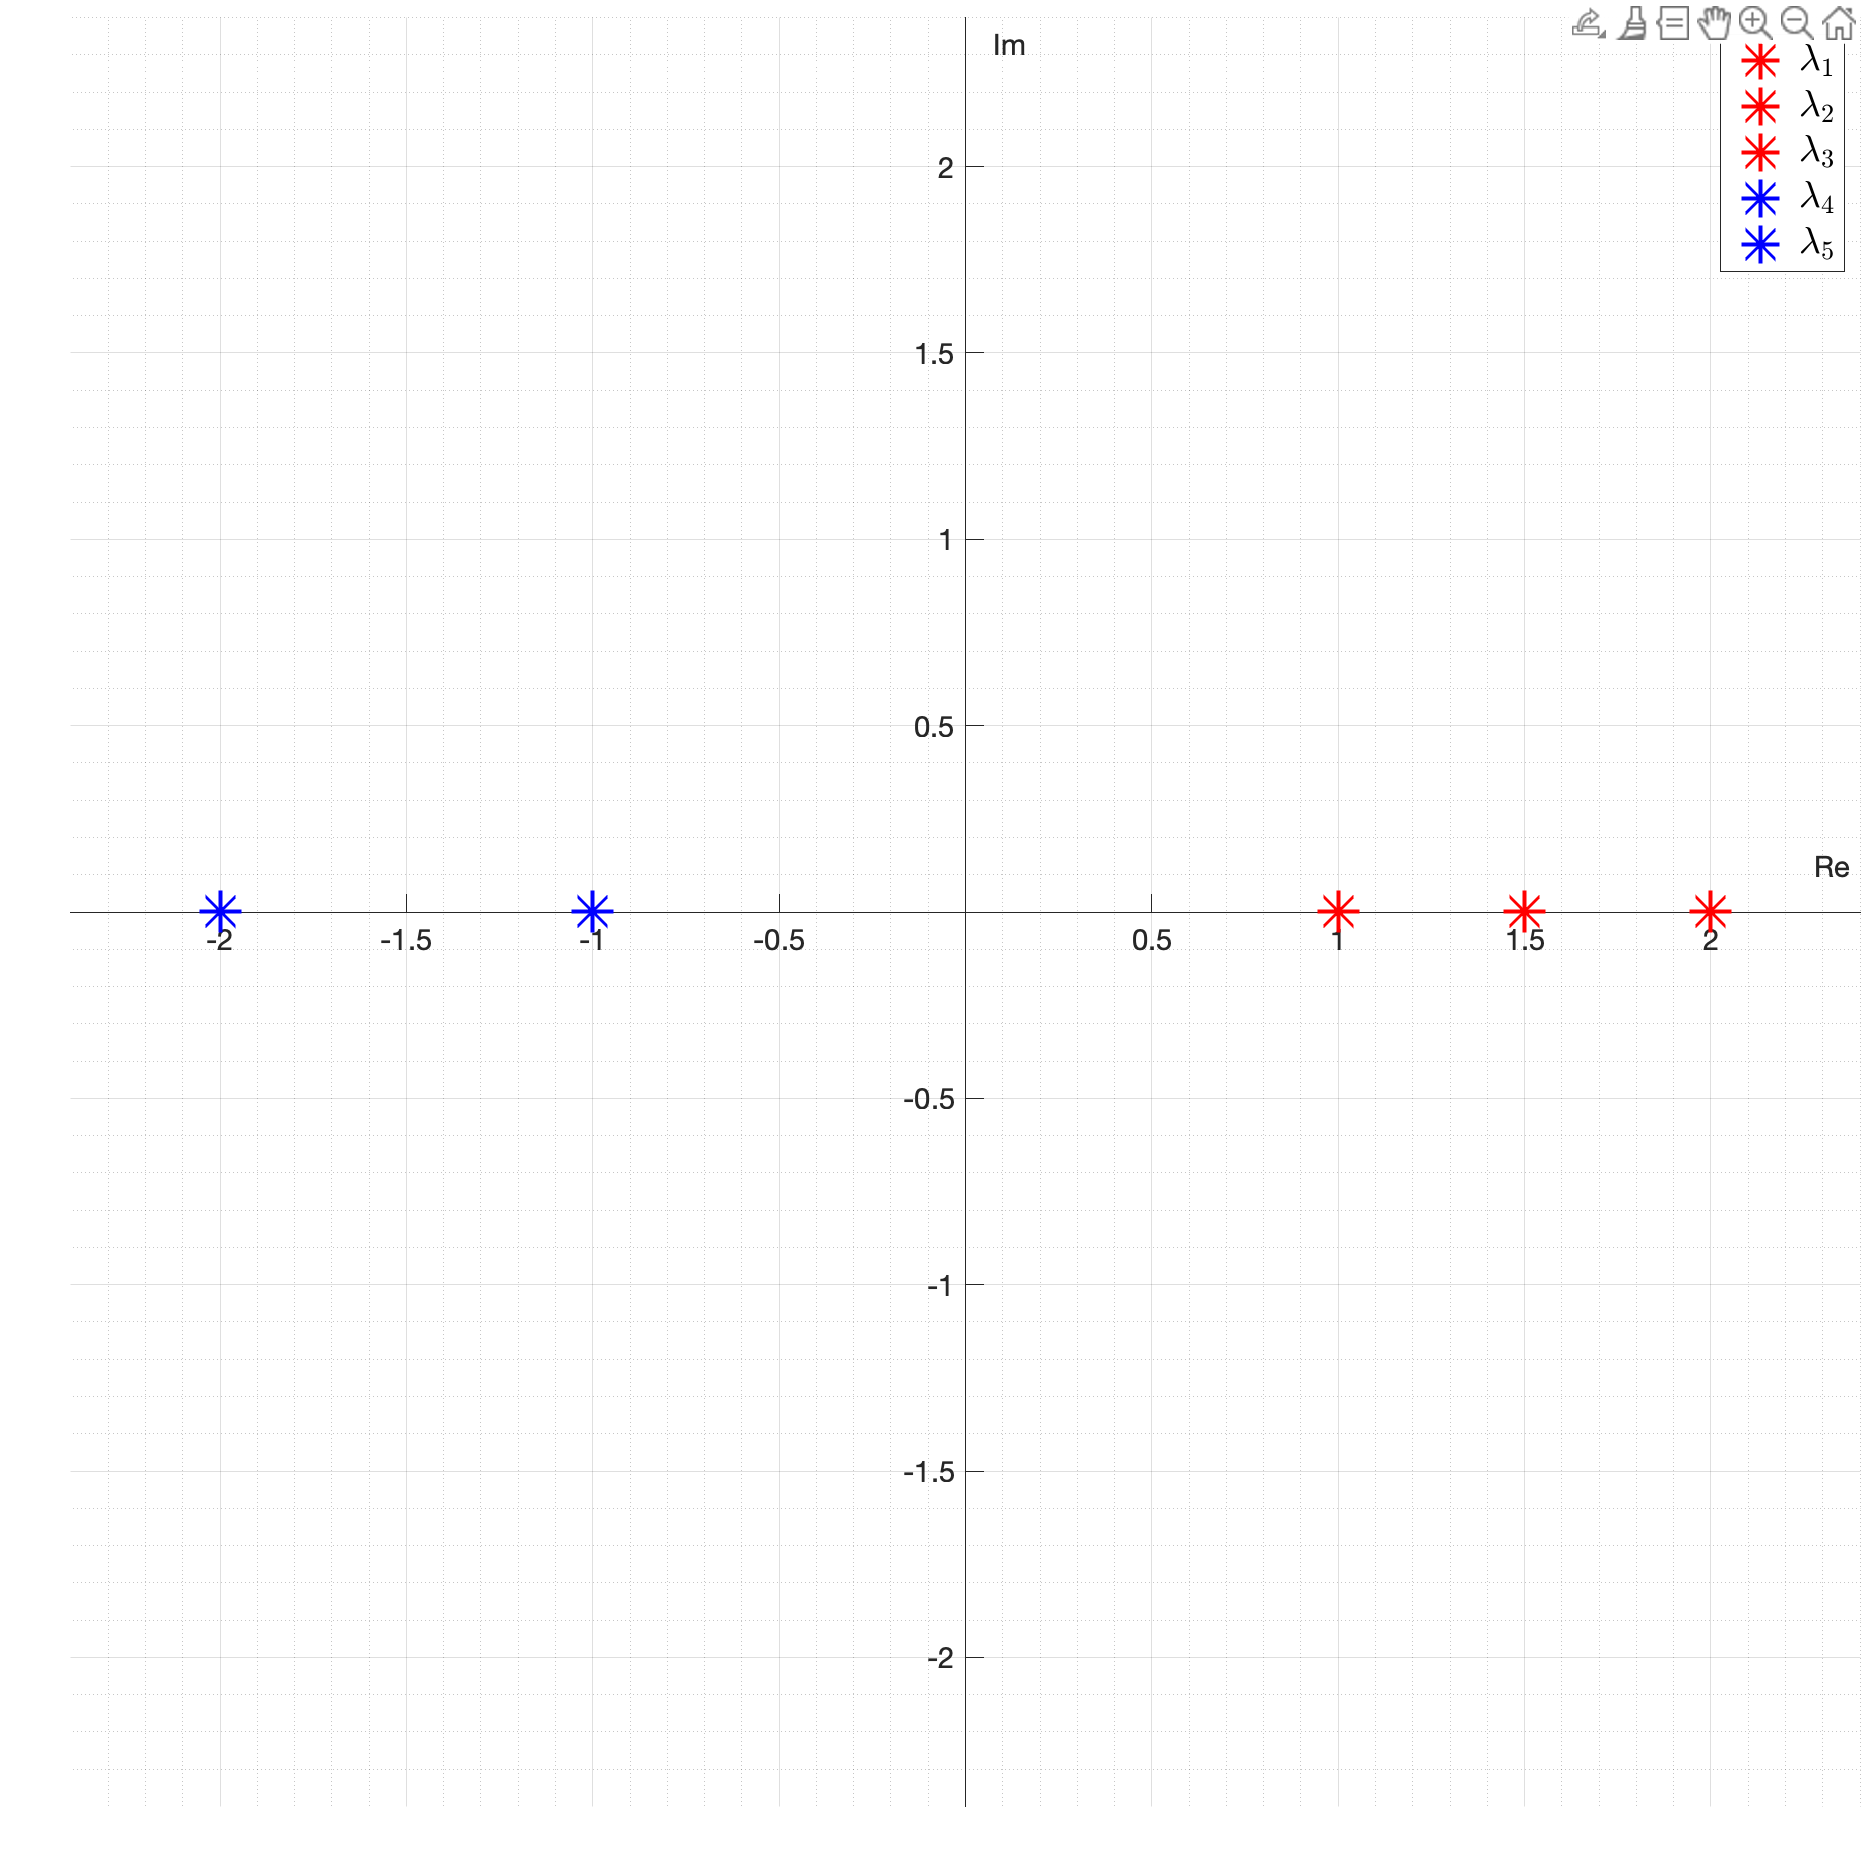
\includegraphics[width=\textwidth]{media/plots/task1_poles_open.png}
        \caption{Разомкнутая система}
        \label{fig:task1_poles:open}
    \end{subfigure}%
    \begin{subfigure}{0.5\textwidth}
        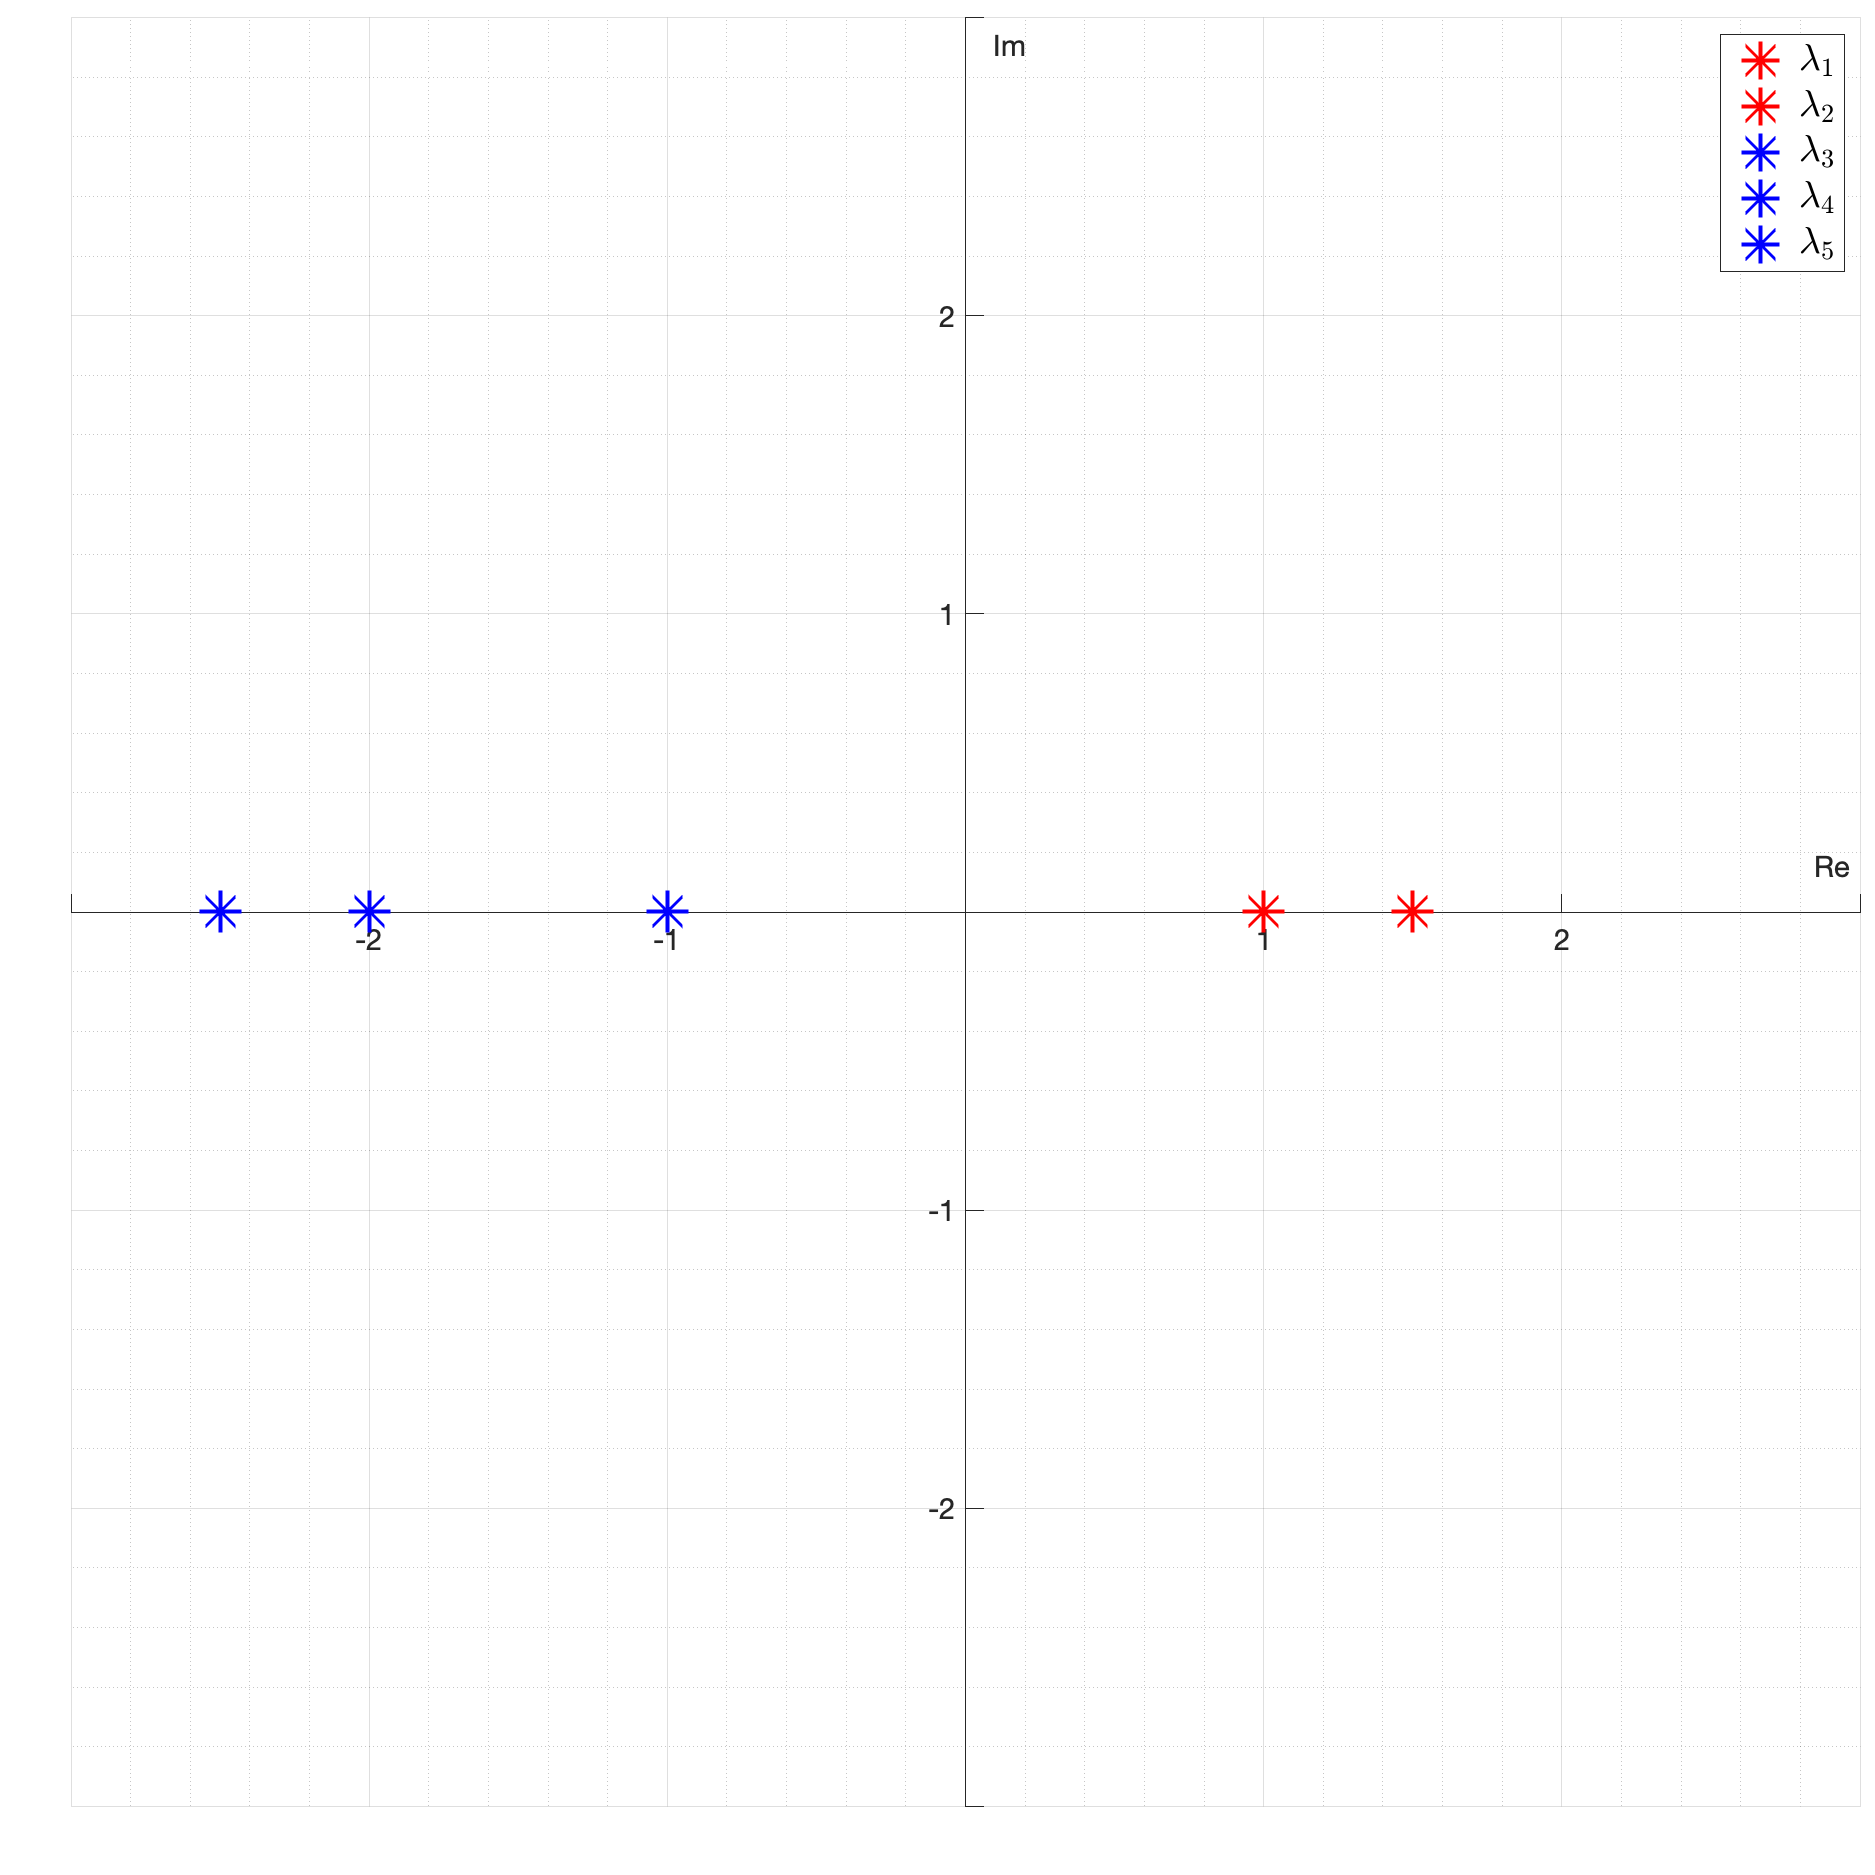
\includegraphics[width=\textwidth]{media/plots/task1_poles_closed.png}
        \caption{Замкнутая система}
        \label{fig:task1_poles:closed}
    \end{subfigure}
    \caption{Карты расположения полюсов}
    \label{fig:task1_poles}
\end{figure}

Переходные характеристики систем приведены на рисунке \ref{fig:task1_respoces}.
\begin{figure}[ht!]
    \centering
    \begin{subfigure}{0.5\textwidth}
        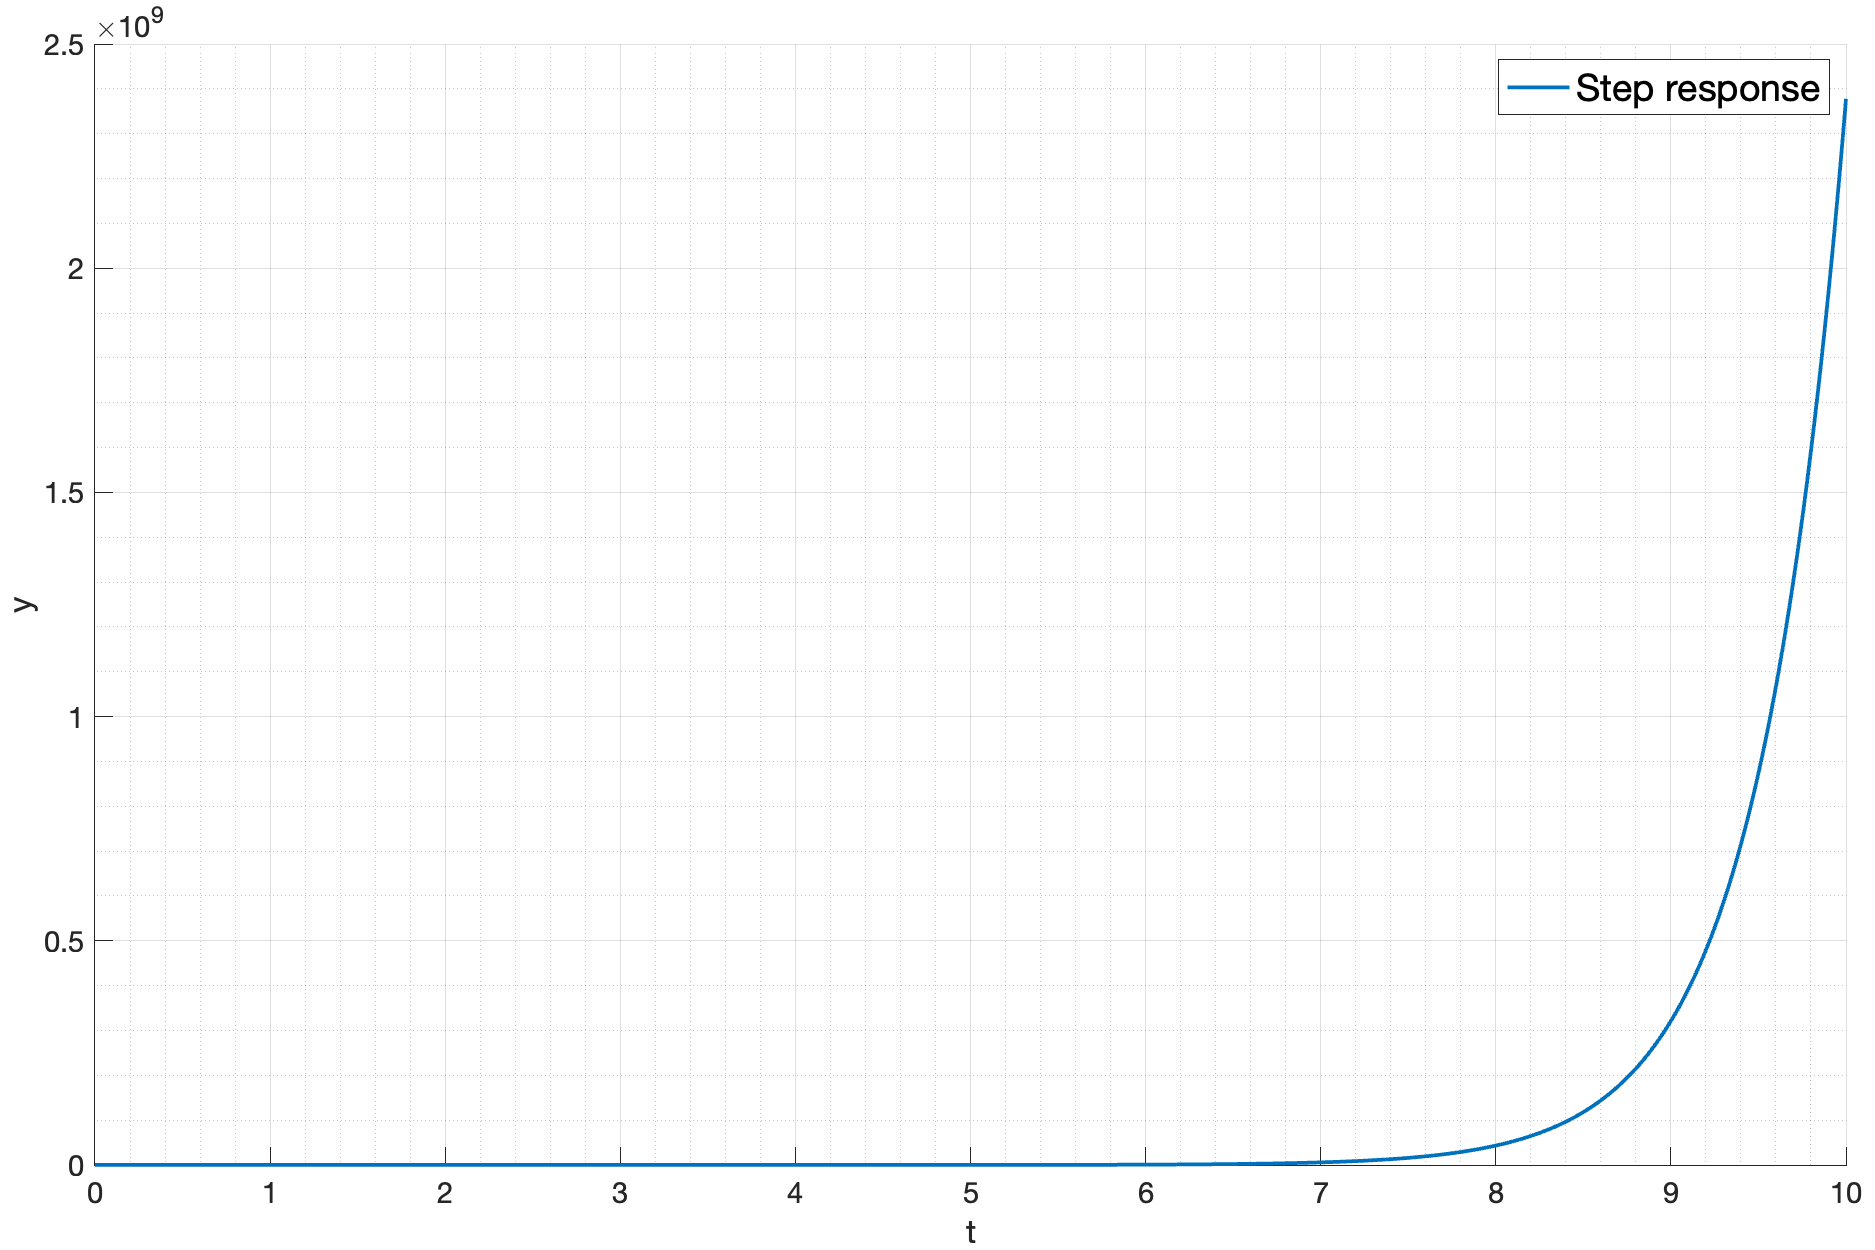
\includegraphics[width=\textwidth]{media/plots/task1_step_response_open.png}
        \caption{Разомкнутая система (переходная)}
        \label{fig:task1_step:open}
    \end{subfigure}%
    \begin{subfigure}{0.5\textwidth}
        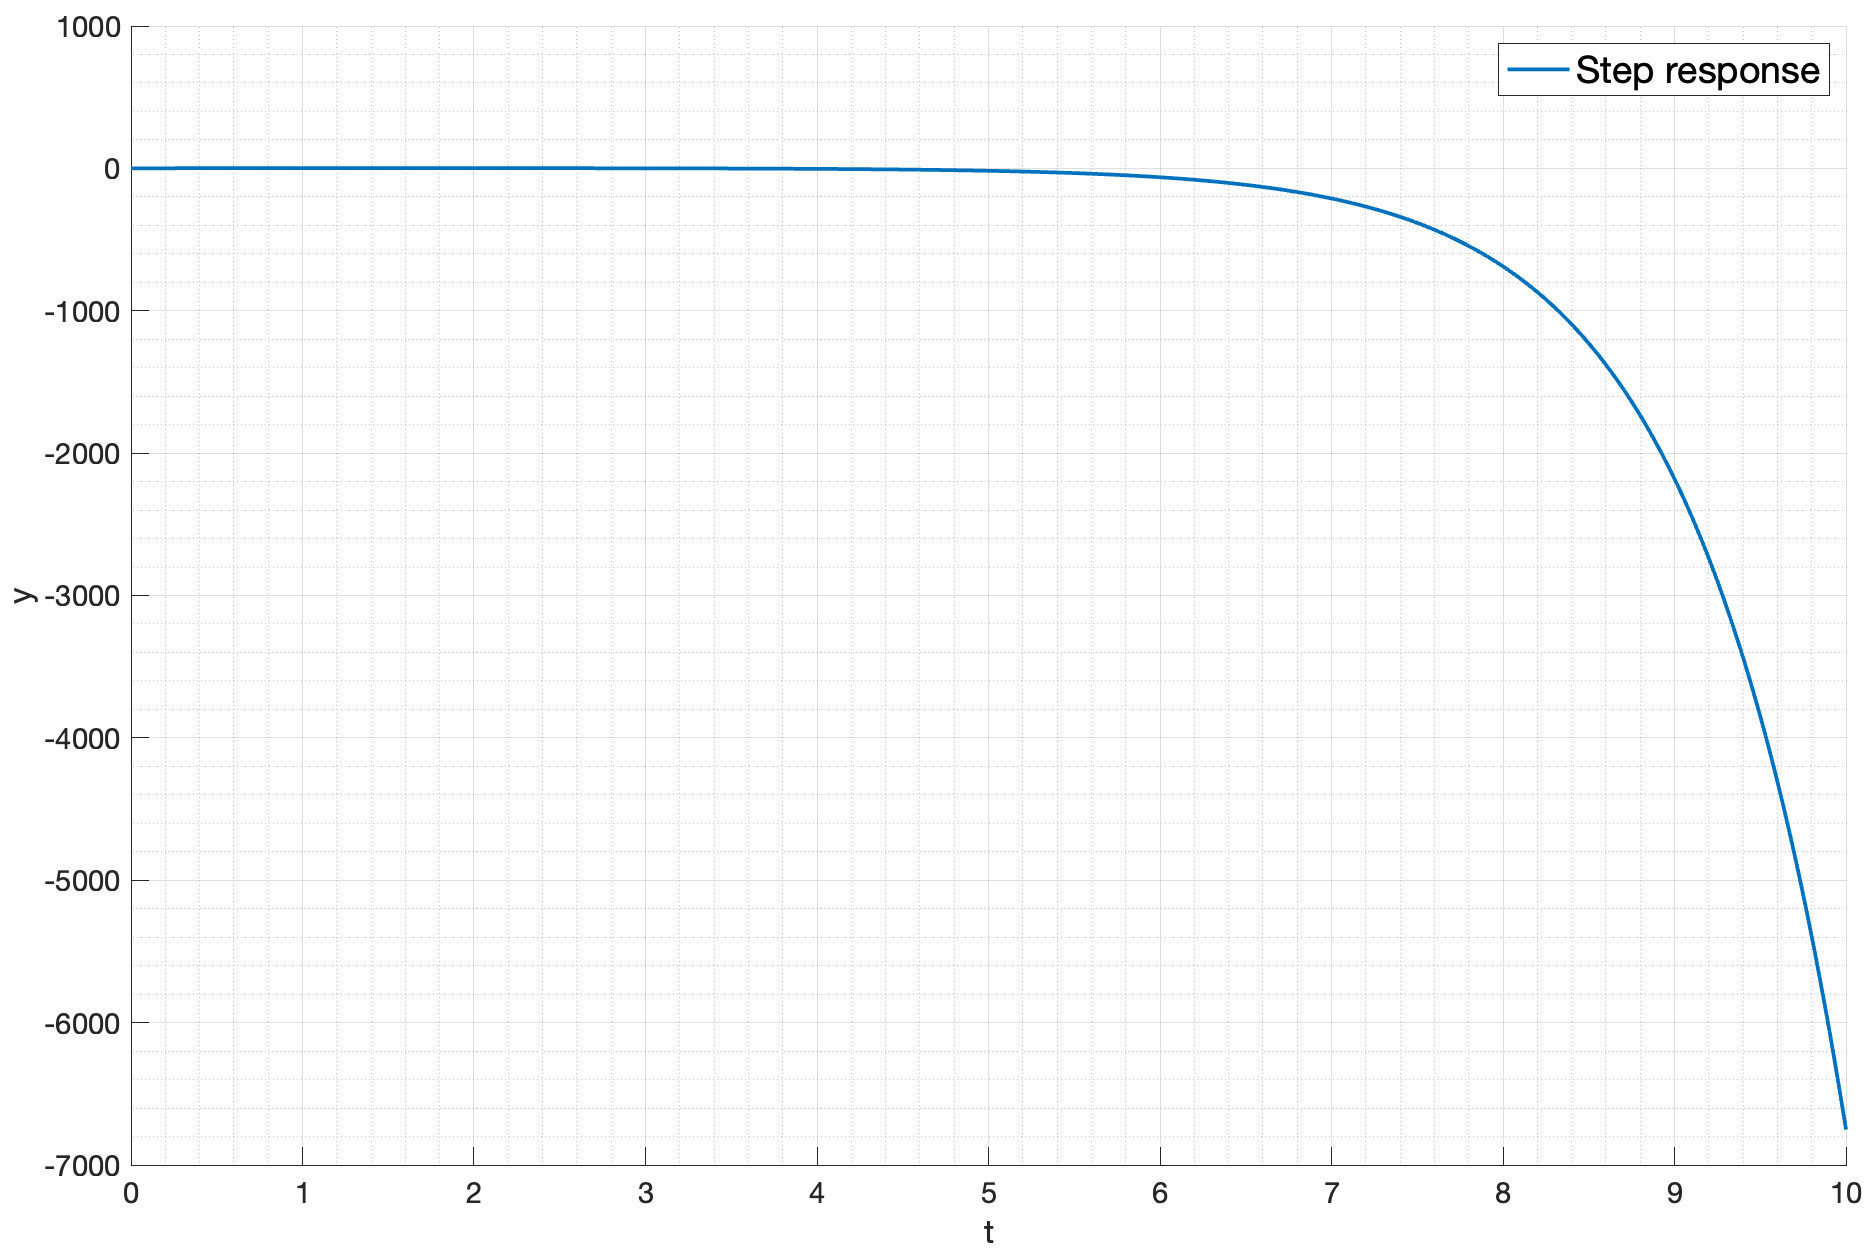
\includegraphics[width=\textwidth]{media/plots/task1_step_response_closed.png}
        \caption{Замкнутая система (переходная)}
        \label{fig:task1_step:closed}
    \end{subfigure}
    \begin{subfigure}{0.5\textwidth}
        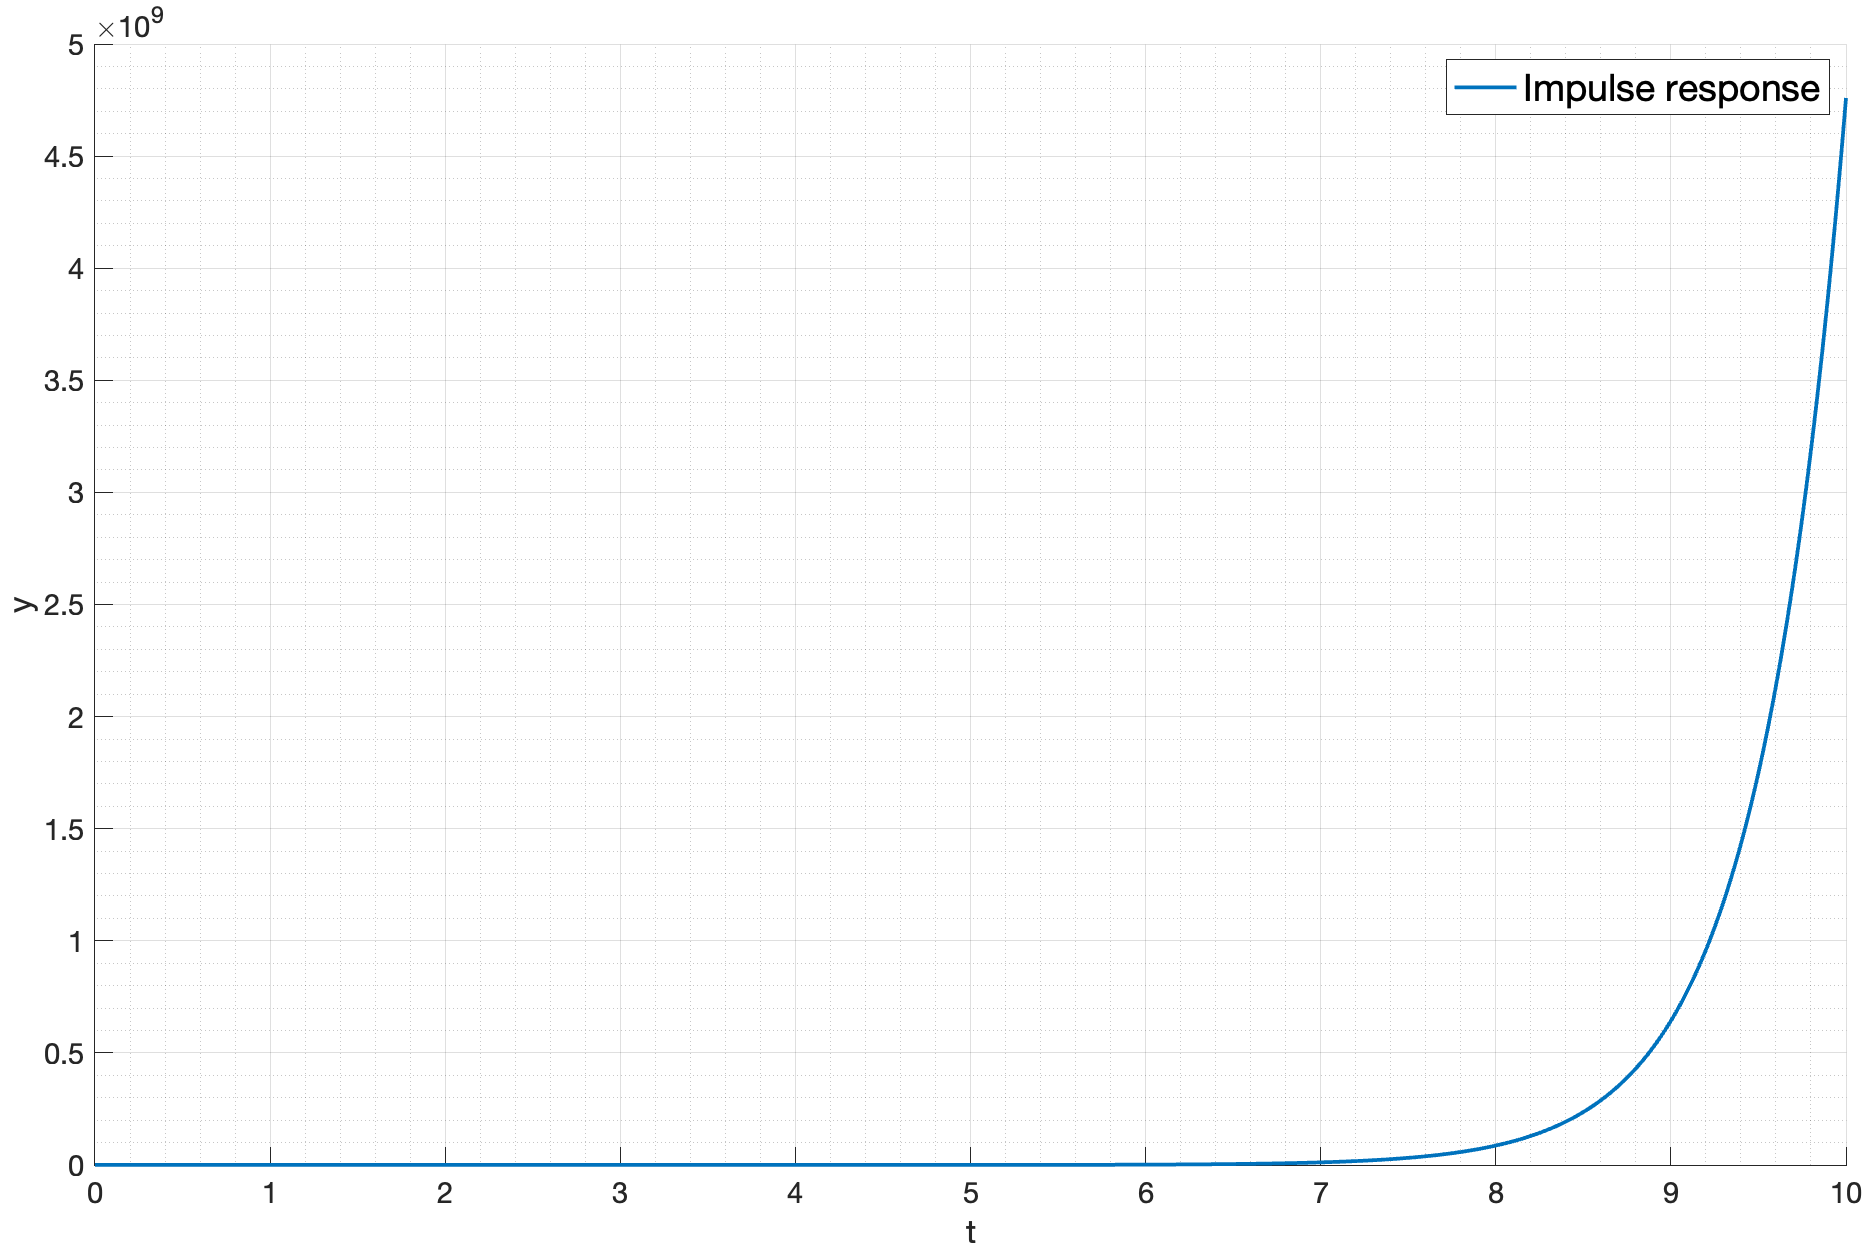
\includegraphics[width=\textwidth]{media/plots/task1_impulse_response_open.png}
        \caption{Замкнутая система (весовая)}
        \label{fig:task1_impulse:open}
    \end{subfigure}%
    \begin{subfigure}{0.5\textwidth}
        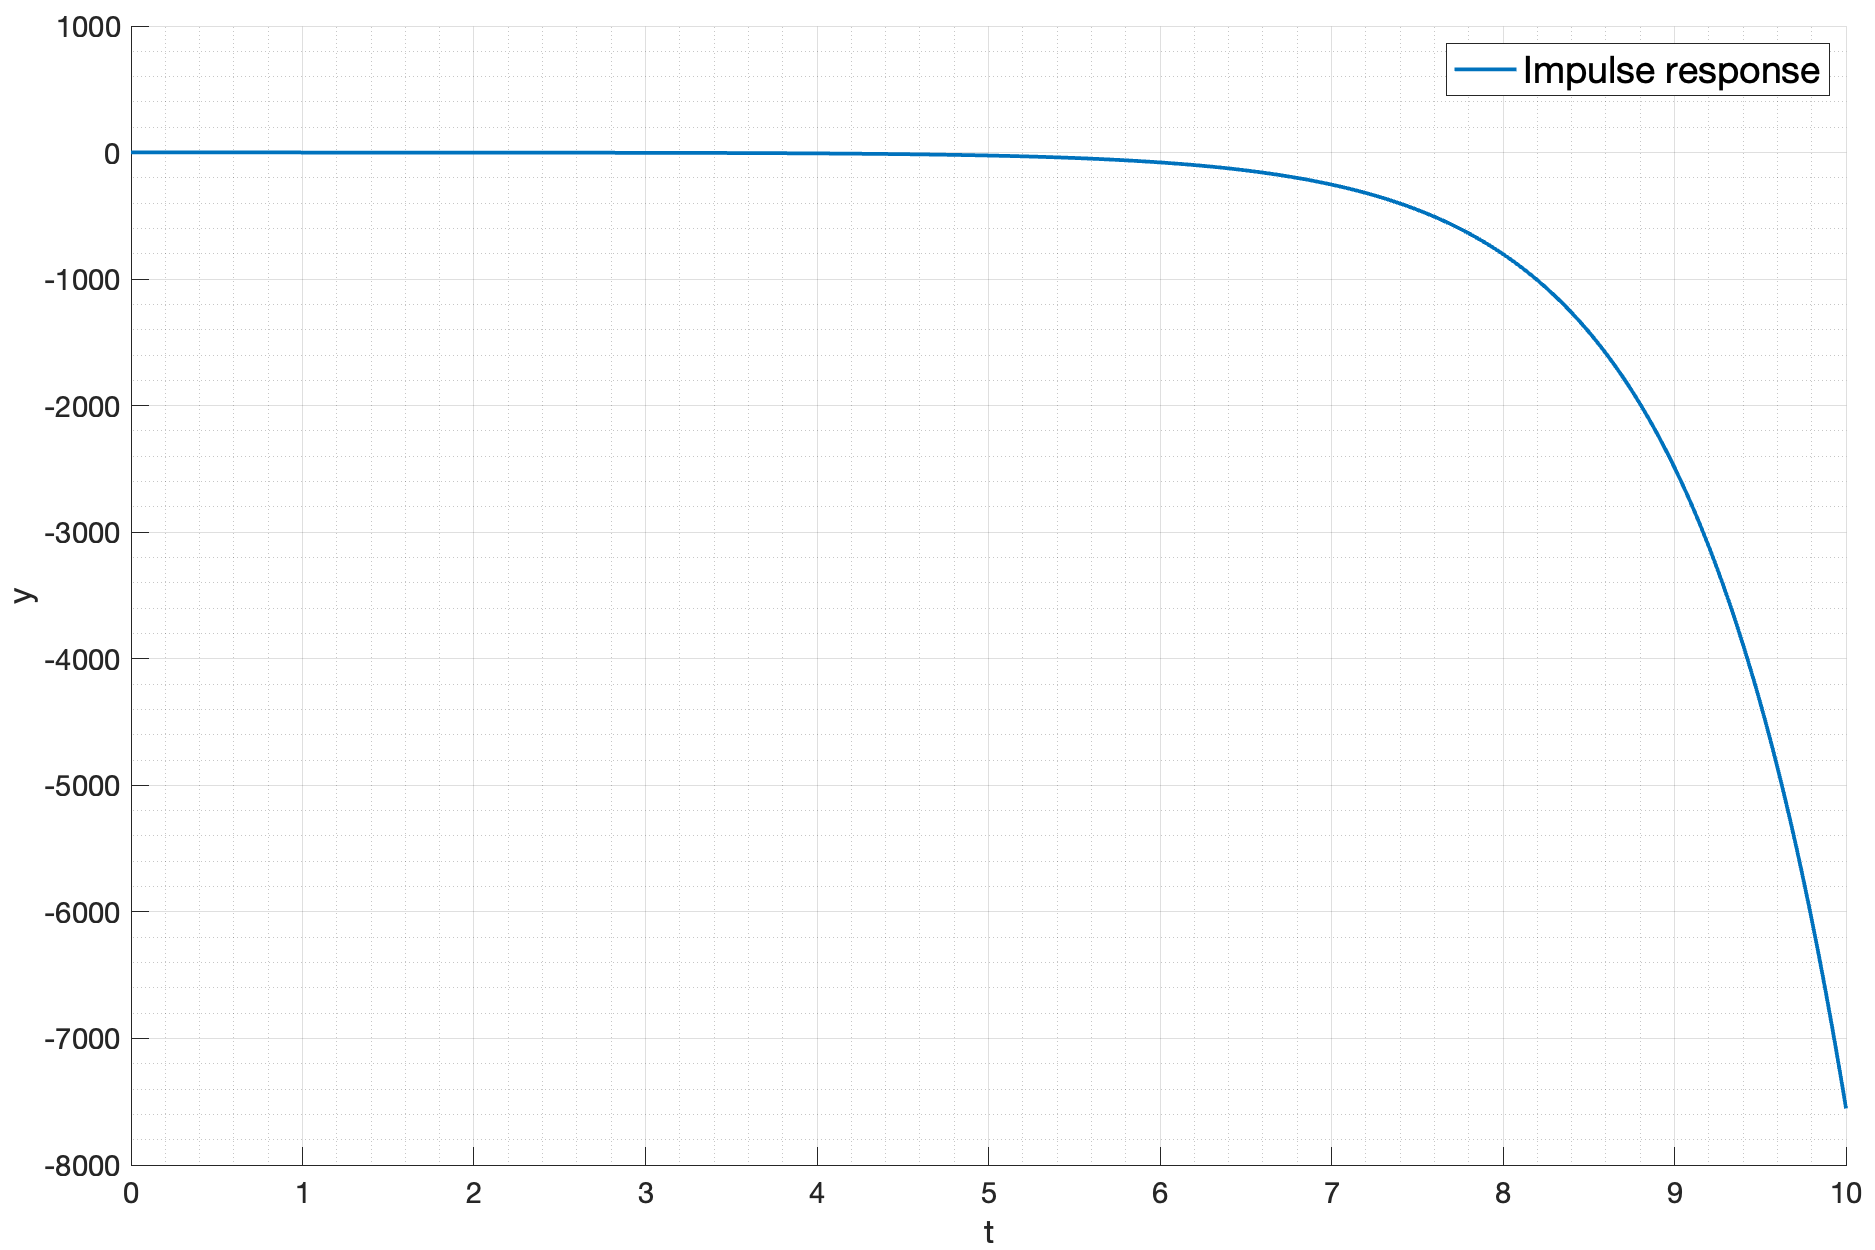
\includegraphics[width=\textwidth]{media/plots/task1_impulse_response_closed.png}
        \caption{Замкнутая система (весовая)}
        \label{fig:task1_impulse:closed}
    \end{subfigure}
    \caption{Переходные характеристики}
    \label{fig:task1_respoces}
\end{figure}

Годограф Найквиста приведен на рисунке \ref{fig:task1_nyquist}.
\begin{figure}[ht!]
    \centering
    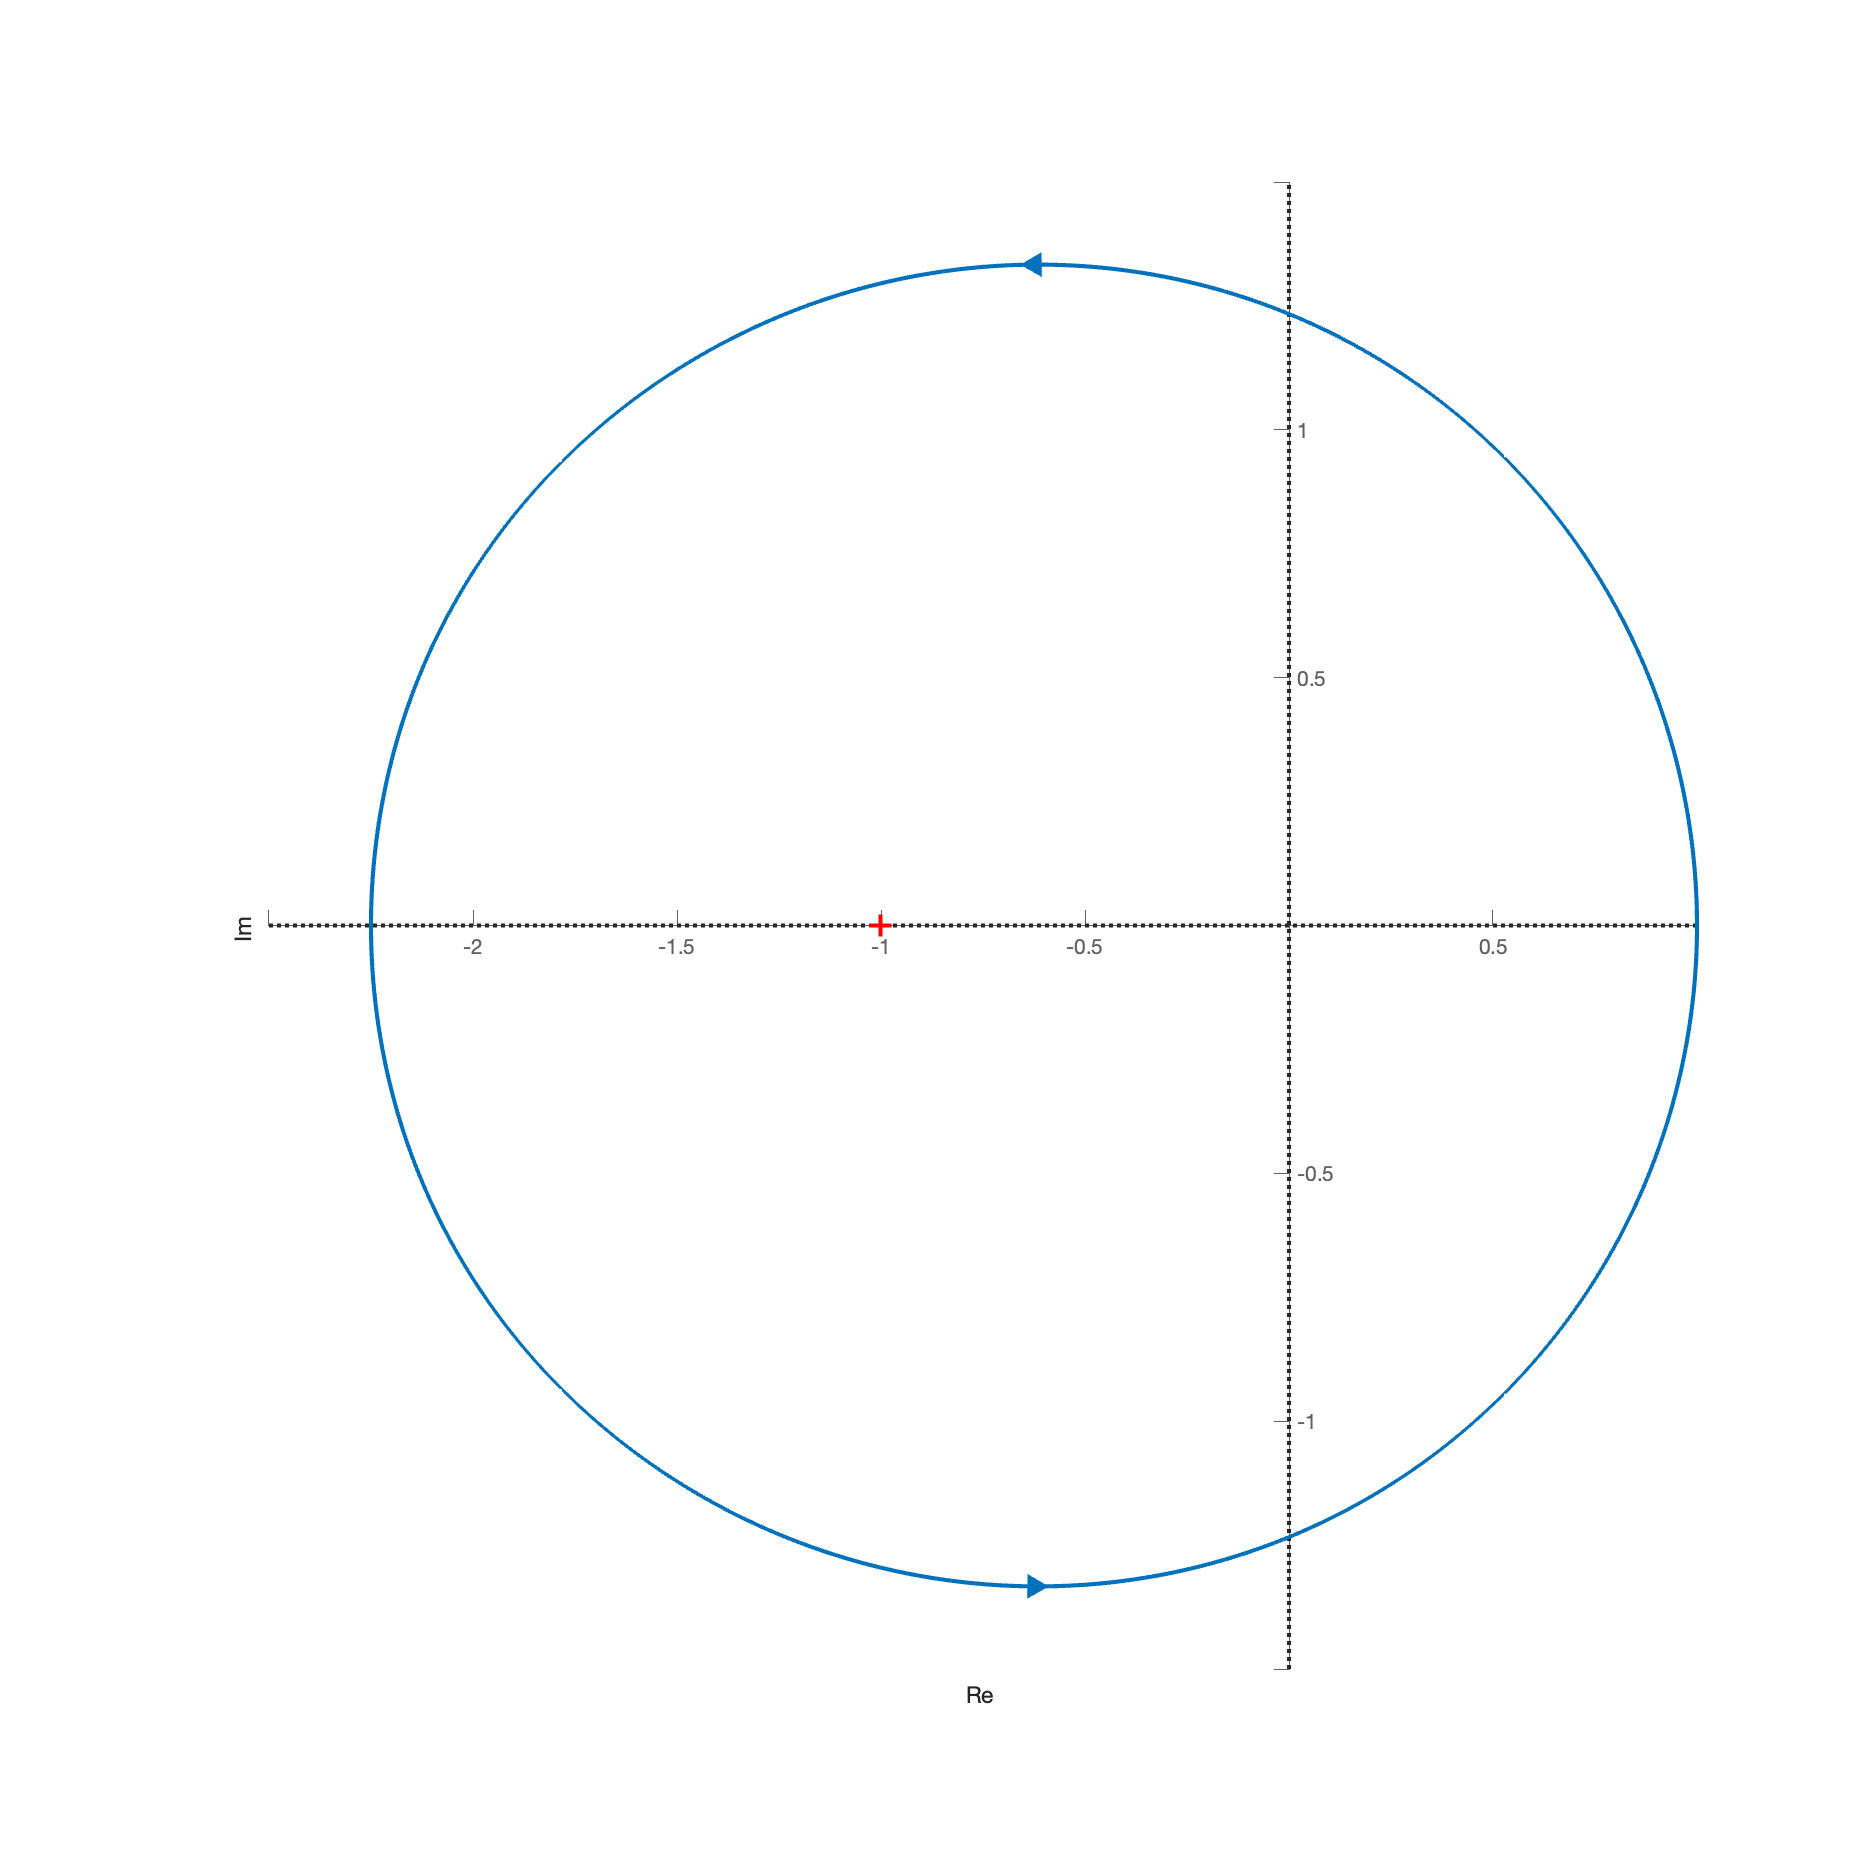
\includegraphics[width=\textwidth]{media/plots/task1_nyquist_open.png}
    \caption{Годограф Найквиста}
    \label{fig:task1_nyquist}
\end{figure}
Найдем количество оборотов годографа вокруг точки $(-1, 0)$ согласно формуле:
\begin{equation}
    M - N = Z 
\end{equation}
где $Z$ -- количество оборотов годографа вокруг точки $(-1, 0)$ по часовой стрелке, $M$ -- количество неустойчивых полюсов замкнутой системы, $N$ -- количество неустойчивых полюсов разомкнутой системы. 
В данном случае $M = 2$, $N = 3$, следовательно $Z = -1$, что подтверждает график на рисунке \ref{fig:task1_nyquist}.

Проведем анализ устойчивости на основе логарифмического критерий Найквиста, построим ЛАФЧХ разомкнутой системы (см. рис. \ref{fig:task1_bode_open}). 
\begin{figure}[ht!]
    \centering
    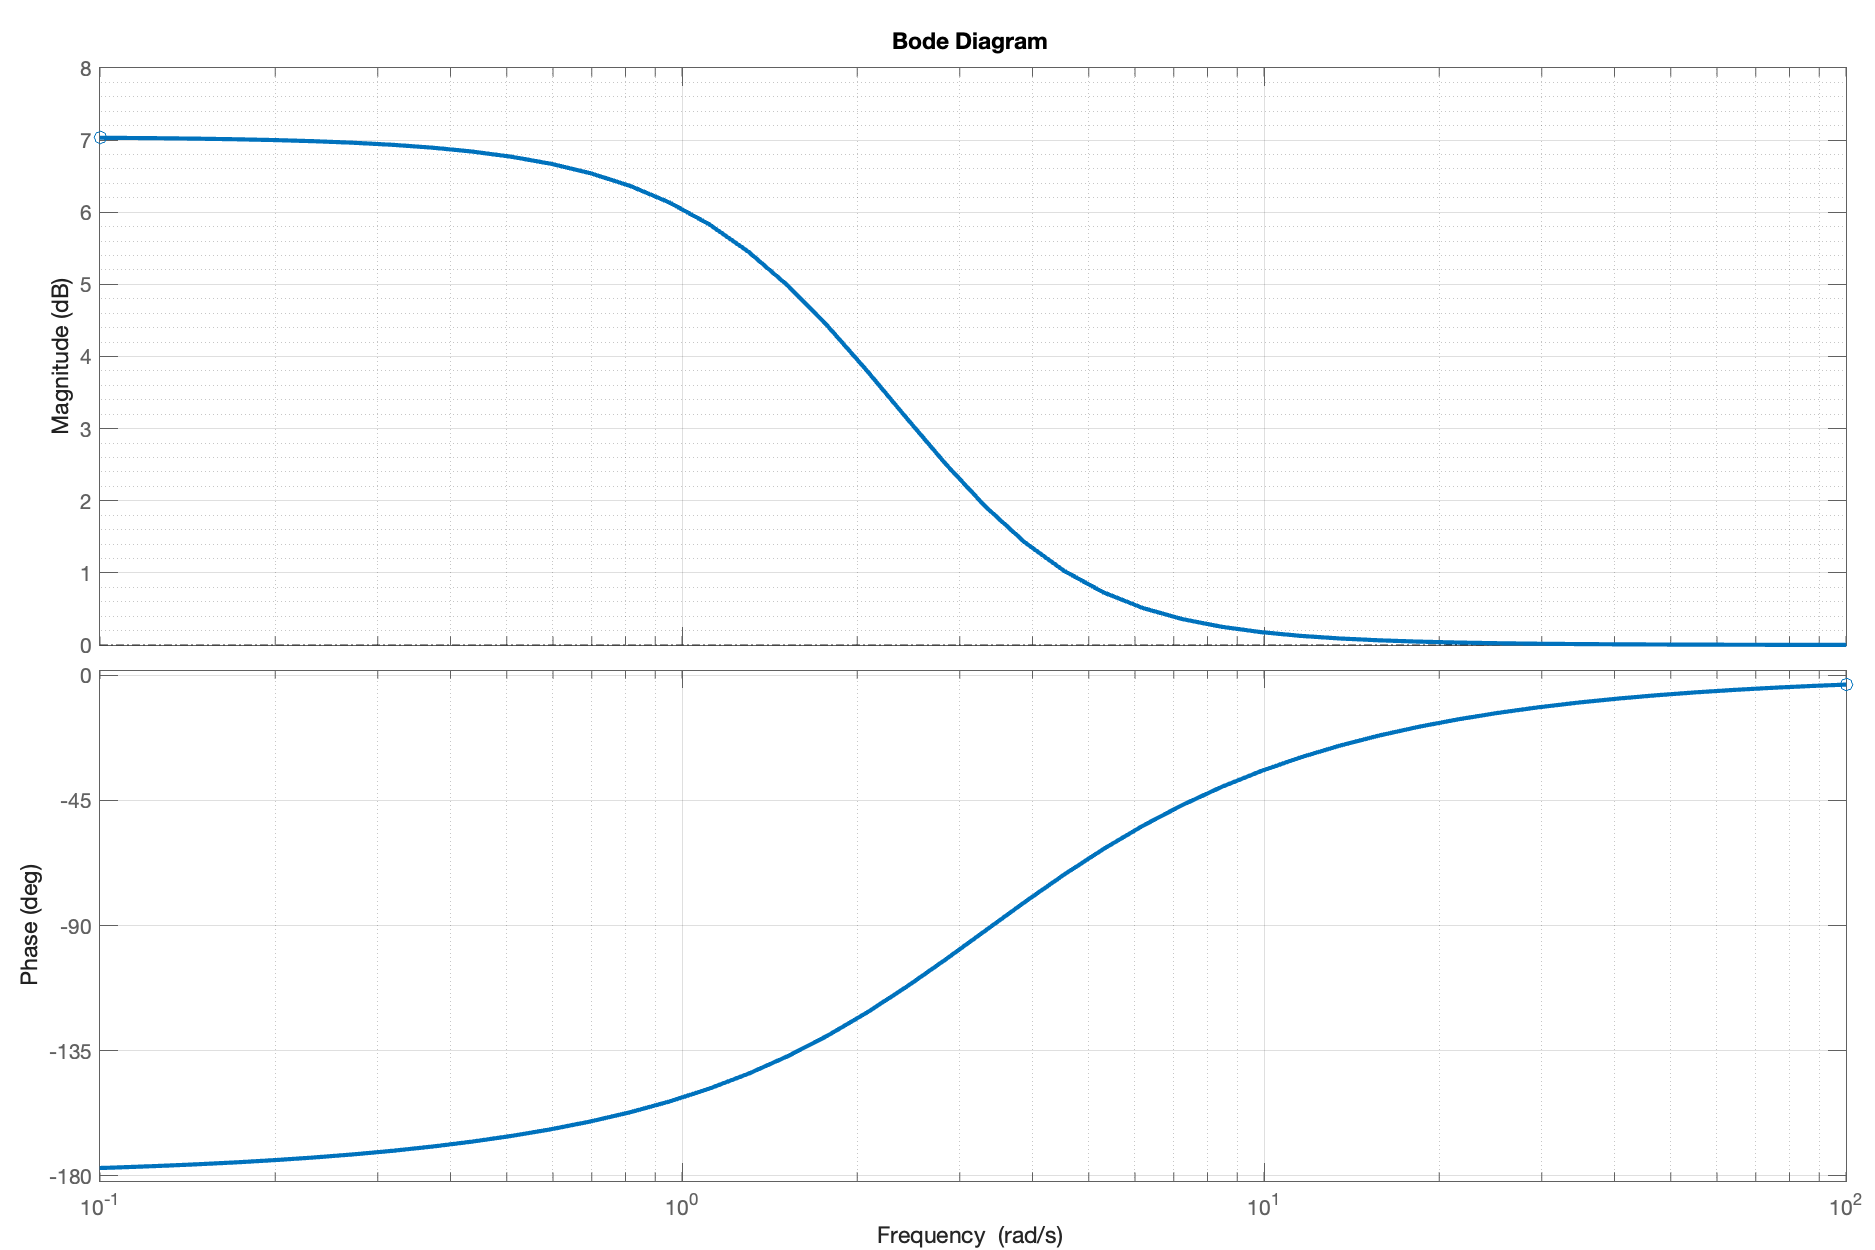
\includegraphics[width=\textwidth]{media/plots/task1_bode_open.png}
    \caption{ЛАФЧХ разомкнутой системы}
    \label{fig:task1_bode_open}
\end{figure}

Так как разомкнутая система имела 3 неустойчивых полюса, нужно, чтобы число переходов через критические точки было равно 1.5. 
На графике видно, что это условие не выполняется, переходы через прямую отсутствуют, но ЛАФЧХ начинается на критическом отрезке, 
значит, сумма переходов будет равна 0.5, что подтверждает \textbf{не}устойчивость системы.

\FloatBarrier
\subsection{Система 2}
Зададимся системой с полюсами $P$:
\begin{equation}
    P = \begin{bmatrix}
        -1 & -1.5 & -2.5 & -3 & -3.5
    \end{bmatrix}
\end{equation}
И полюсами замкнутой системы $K$:
\begin{equation}
    K = \begin{bmatrix}
        -1 & -1.5 & -2.5 & 3 & 3.5
    \end{bmatrix}
\end{equation}

Запишем передаточные функции разомкнутой и замкнутой системы:
\begin{equation}
    W_{\text{o}} = \frac{s^5 -13.00s^4 -65.00s^3 -100.75s^2 -48.75s +0.00}{s^5 +11.50s^4 +50.75s^3 +106.62s^2 +105.75s +39.38}
\end{equation}
\begin{equation}
    W_{\text{c}} = \frac{s^5 -13.00s^4 -65.00s^3 -100.75s^2 -48.75s +0.00}{2s^5 -1.50s^4 -14.25s^3 +5.88s^2 +57.00s +39.38}
\end{equation}

Карты расположения полюсов передаточных функций приведены на рисунках \ref{fig:task2_poles:open} и \ref{fig:task2_poles:closed} соответственно.
\begin{figure}
    \centering
    \begin{subfigure}{0.5\textwidth}
        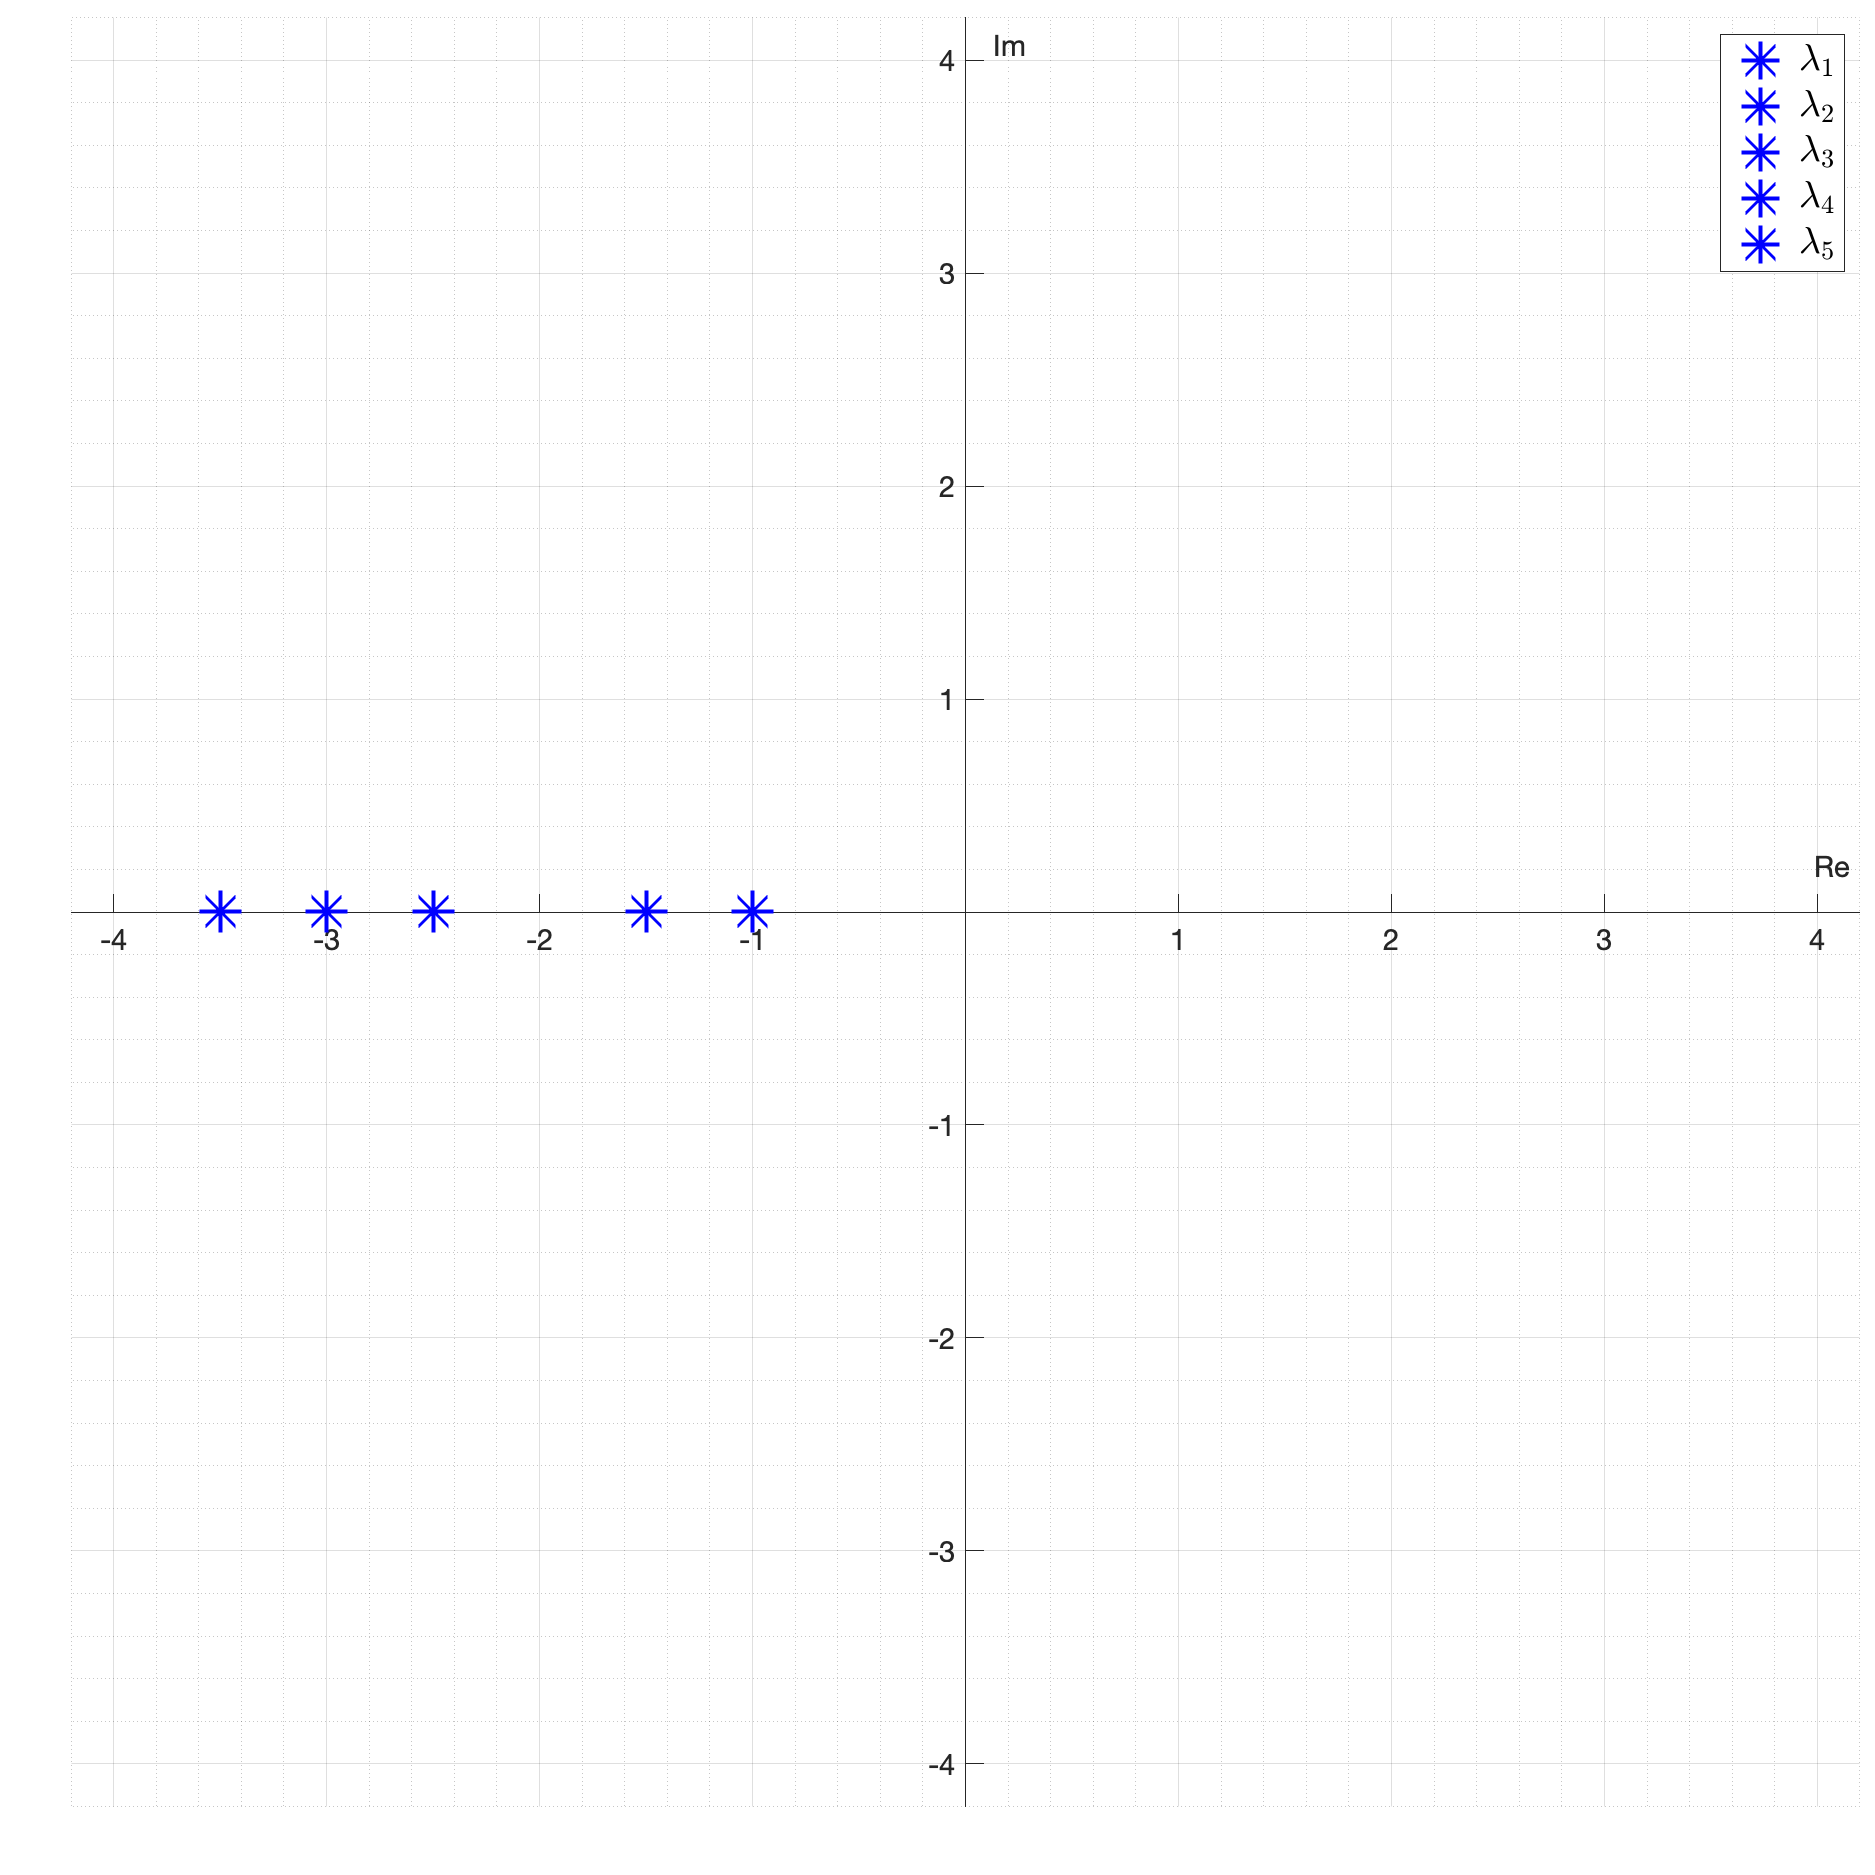
\includegraphics[width=\textwidth]{media/plots/task2_poles_open.png}
        \caption{Разомкнутая система}
        \label{fig:task2_poles:open}
    \end{subfigure}%
    \begin{subfigure}{0.5\textwidth}
        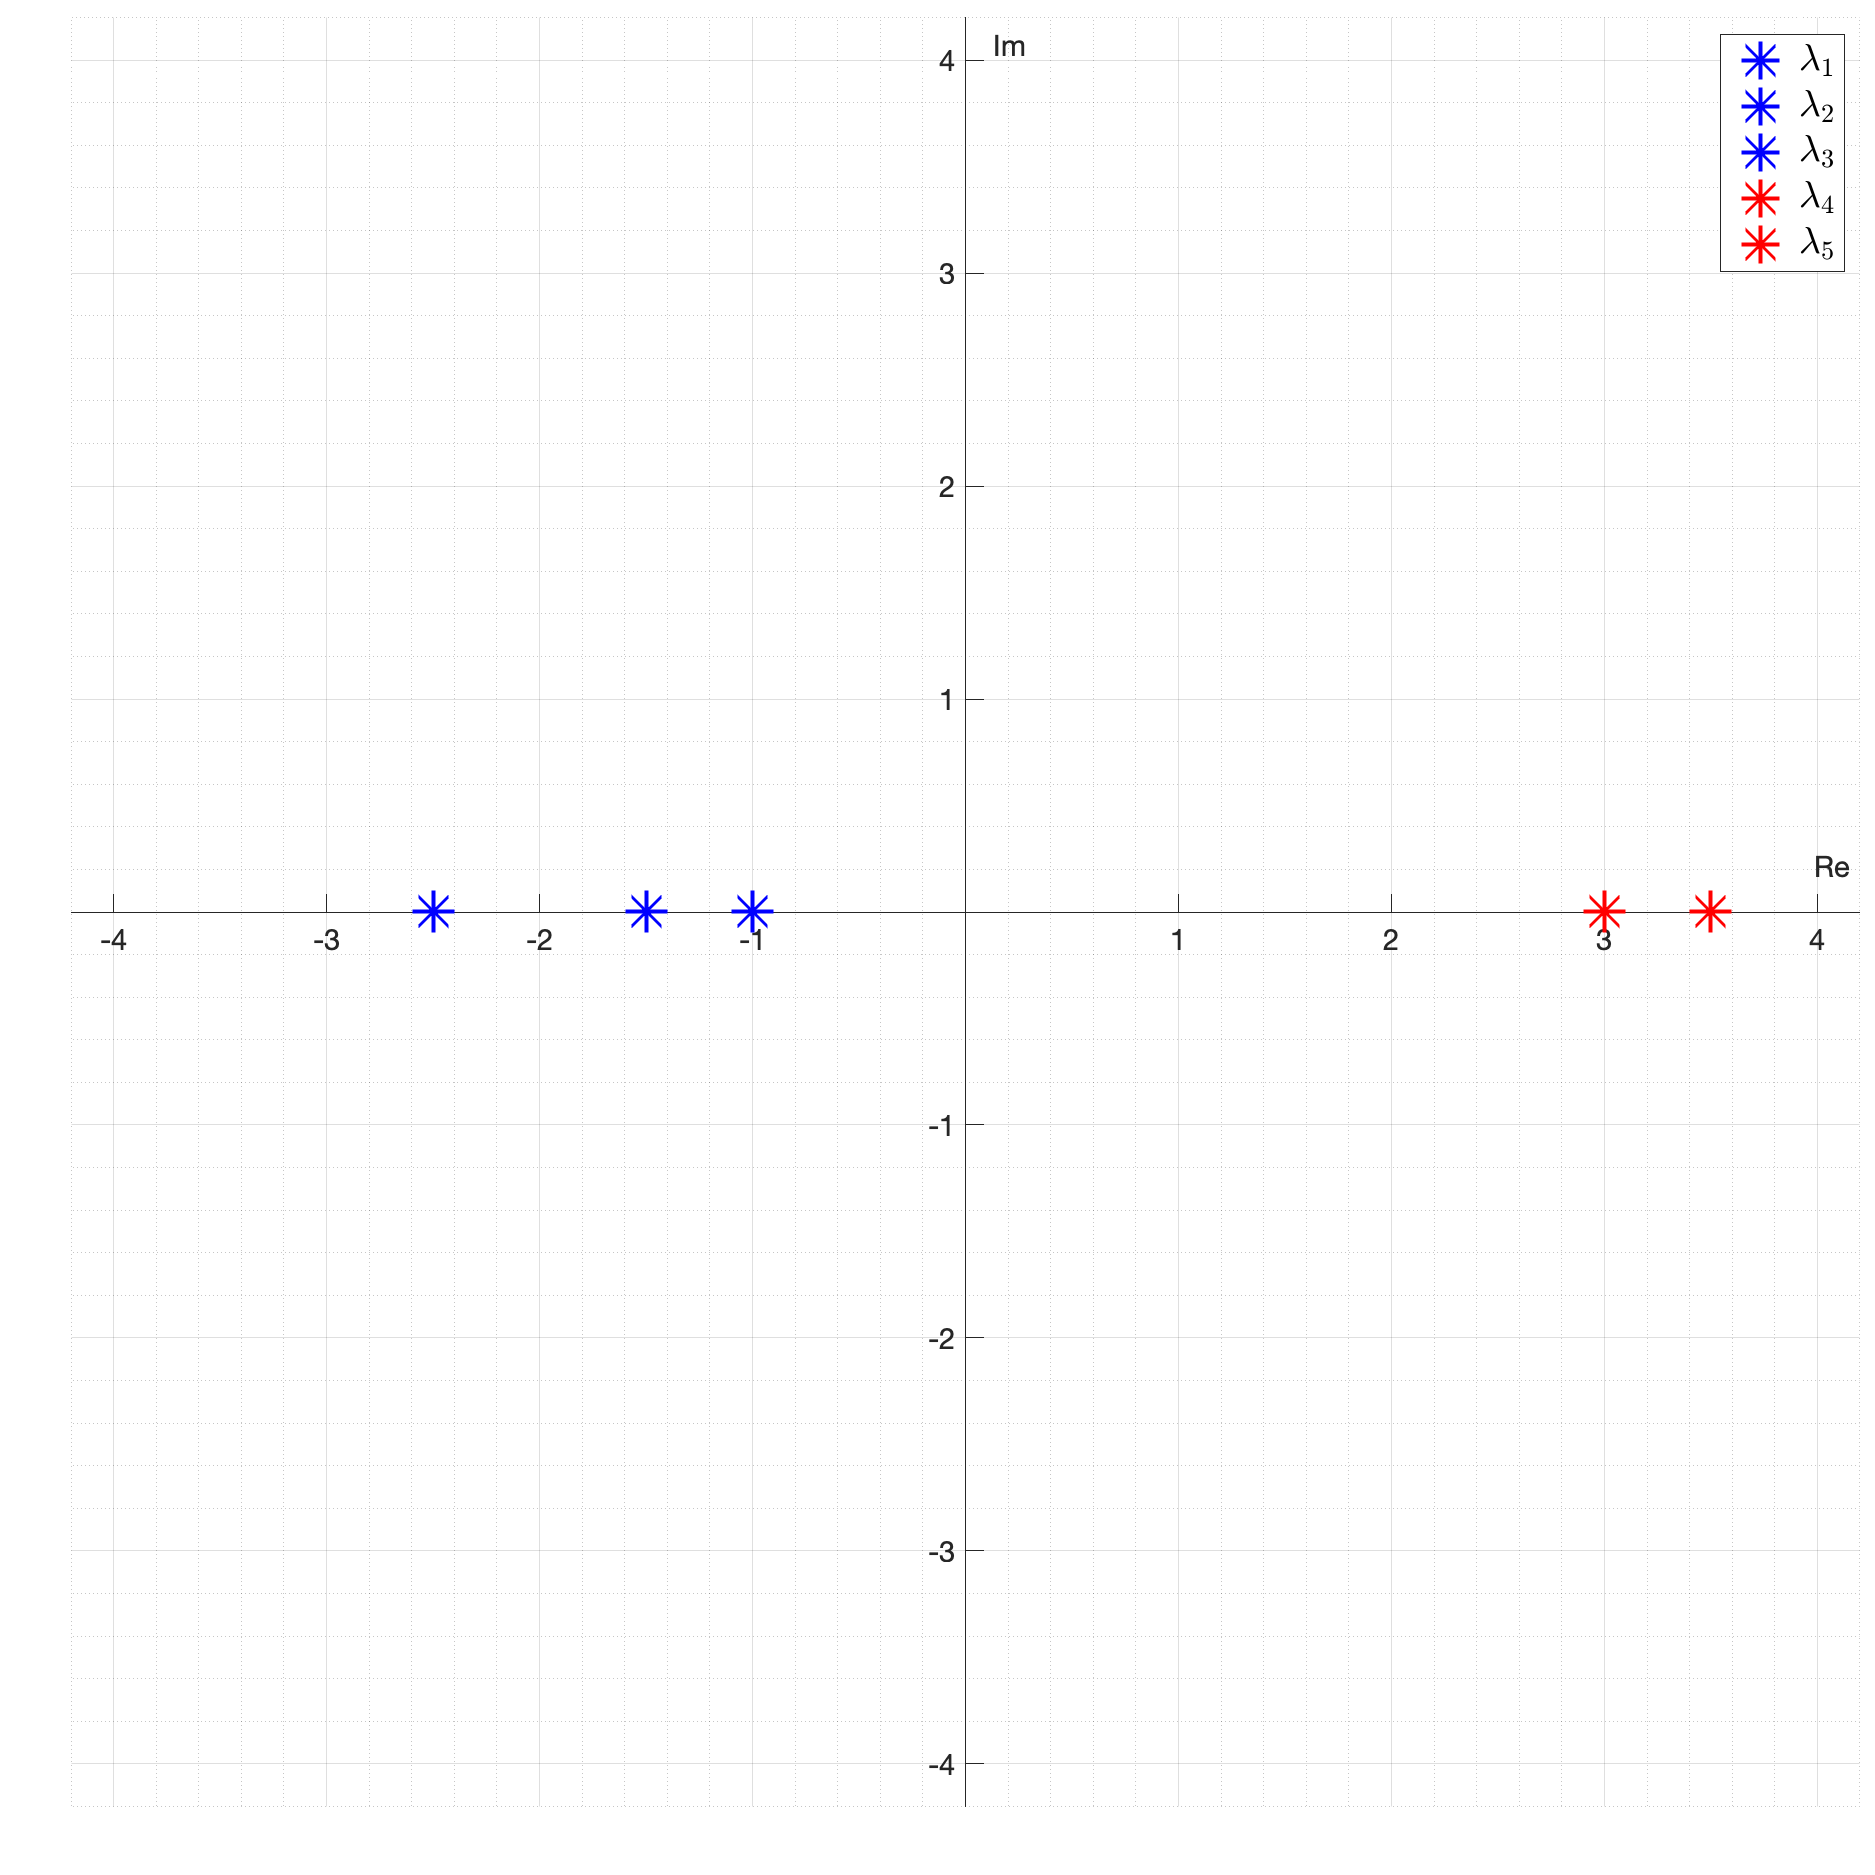
\includegraphics[width=\textwidth]{media/plots/task2_poles_closed.png}
        \caption{Замкнутая система}
        \label{fig:task2_poles:closed}
    \end{subfigure}
    \caption{Карты расположения полюсов}
    \label{fig:task2_poles}
\end{figure}

Переходные характеристики систем приведены на рисунке \ref{fig:task2_respoces}.
\begin{figure}[ht!]
    \centering
    \begin{subfigure}{0.5\textwidth}
        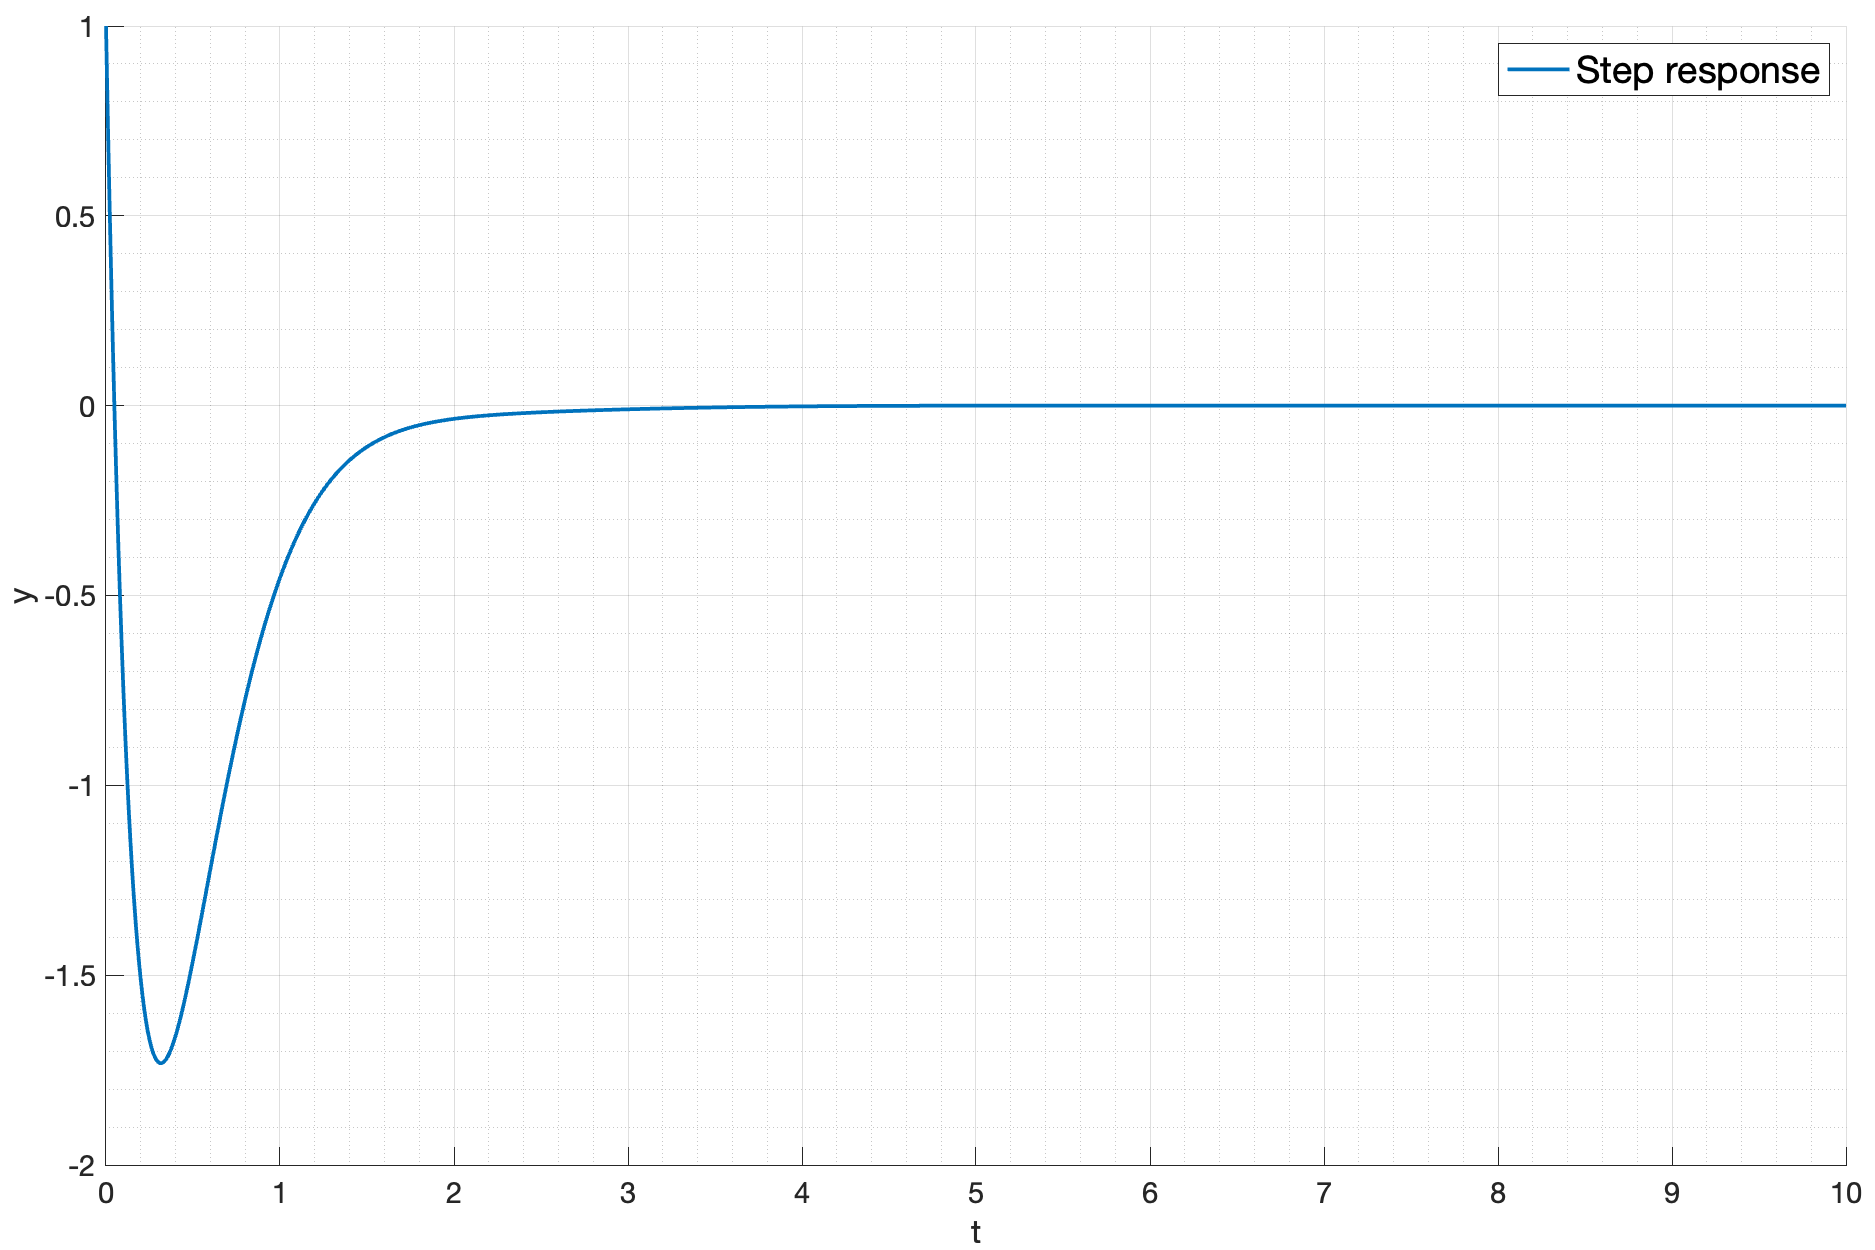
\includegraphics[width=\textwidth]{media/plots/task2_step_response_open.png}
        \caption{Разомкнутая система (переходная)}
        \label{fig:task2_step:open}
    \end{subfigure}%
    \begin{subfigure}{0.5\textwidth}
        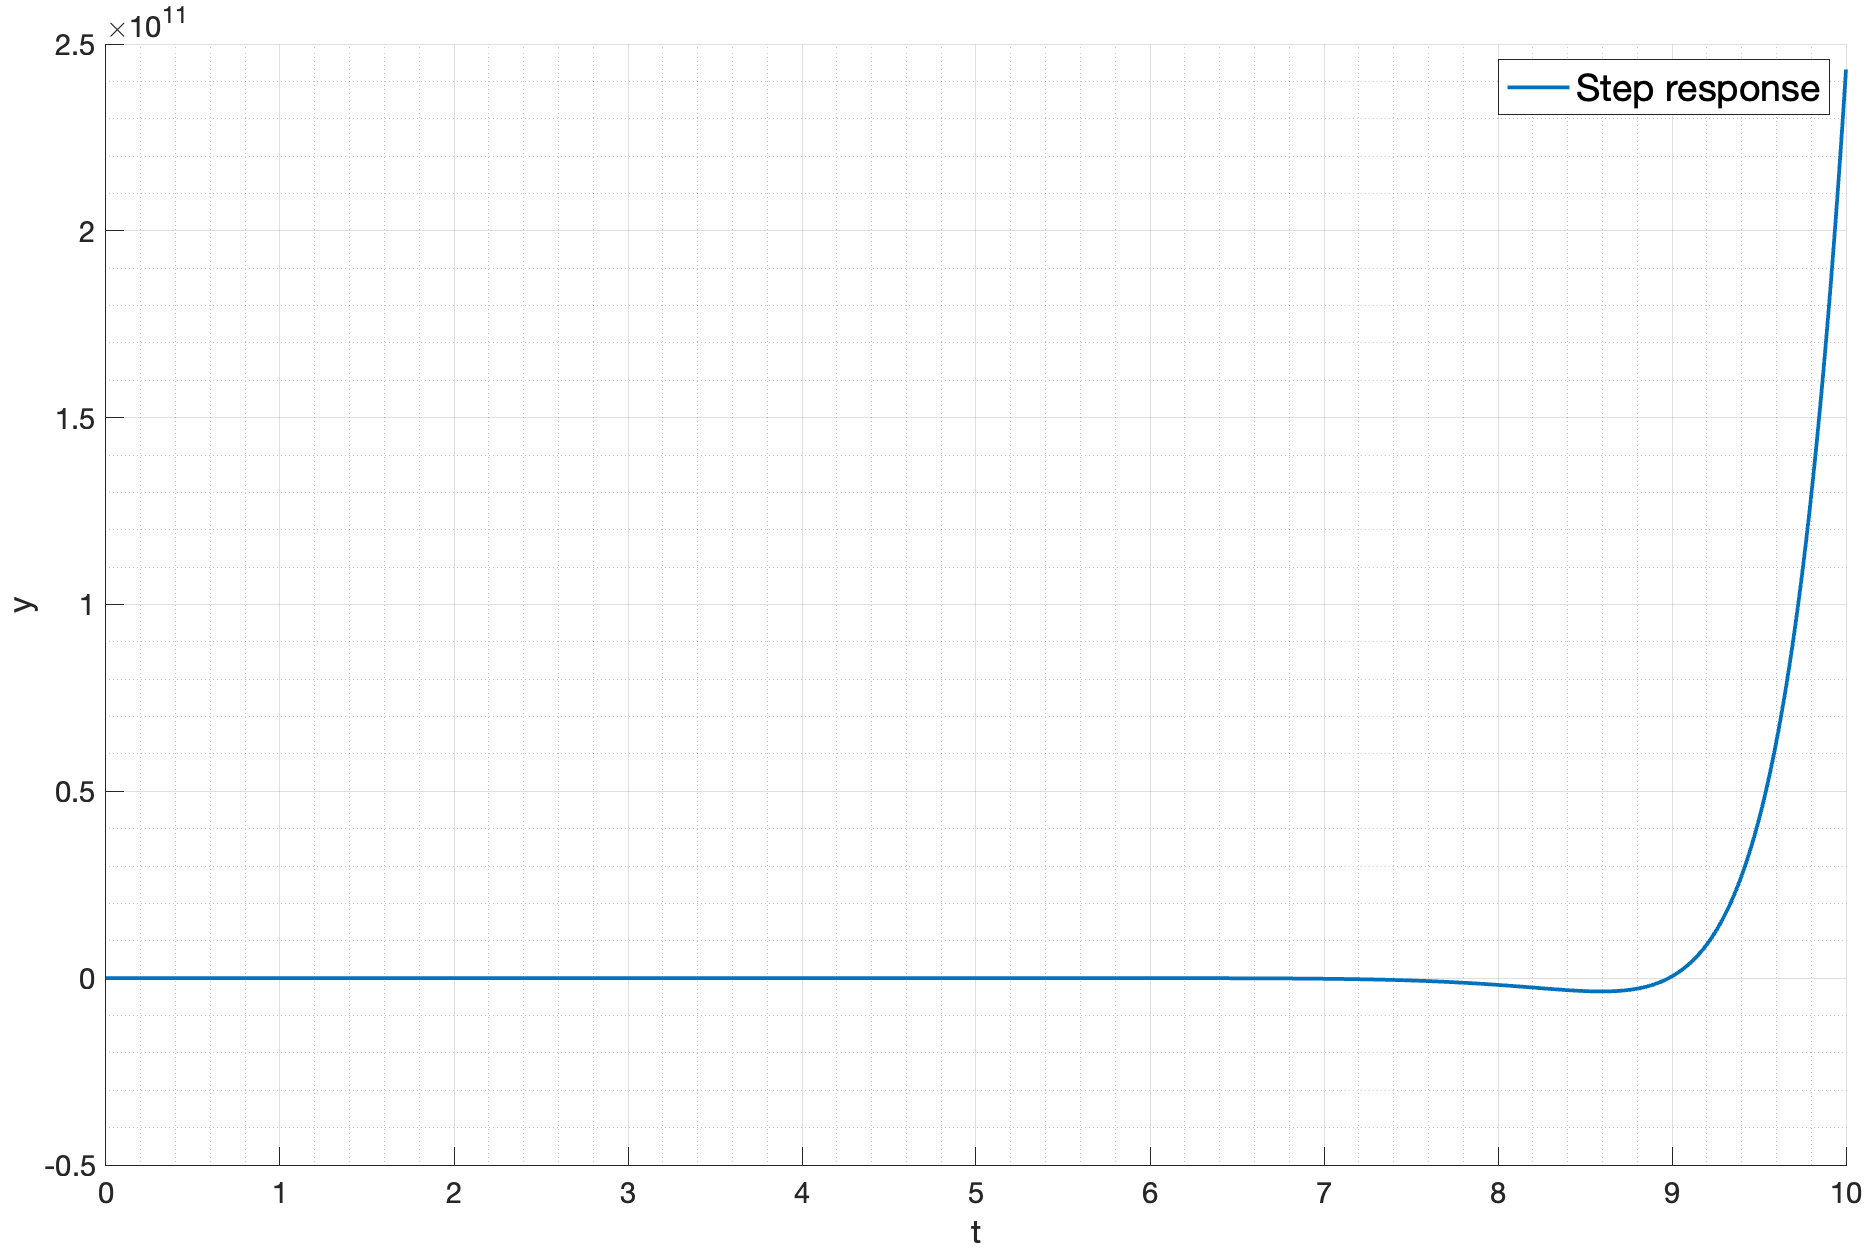
\includegraphics[width=\textwidth]{media/plots/task2_step_response_closed.png}
        \caption{Замкнутая система (переходная)}
        \label{fig:task2_step:closed}
    \end{subfigure}
    \begin{subfigure}{0.5\textwidth}
        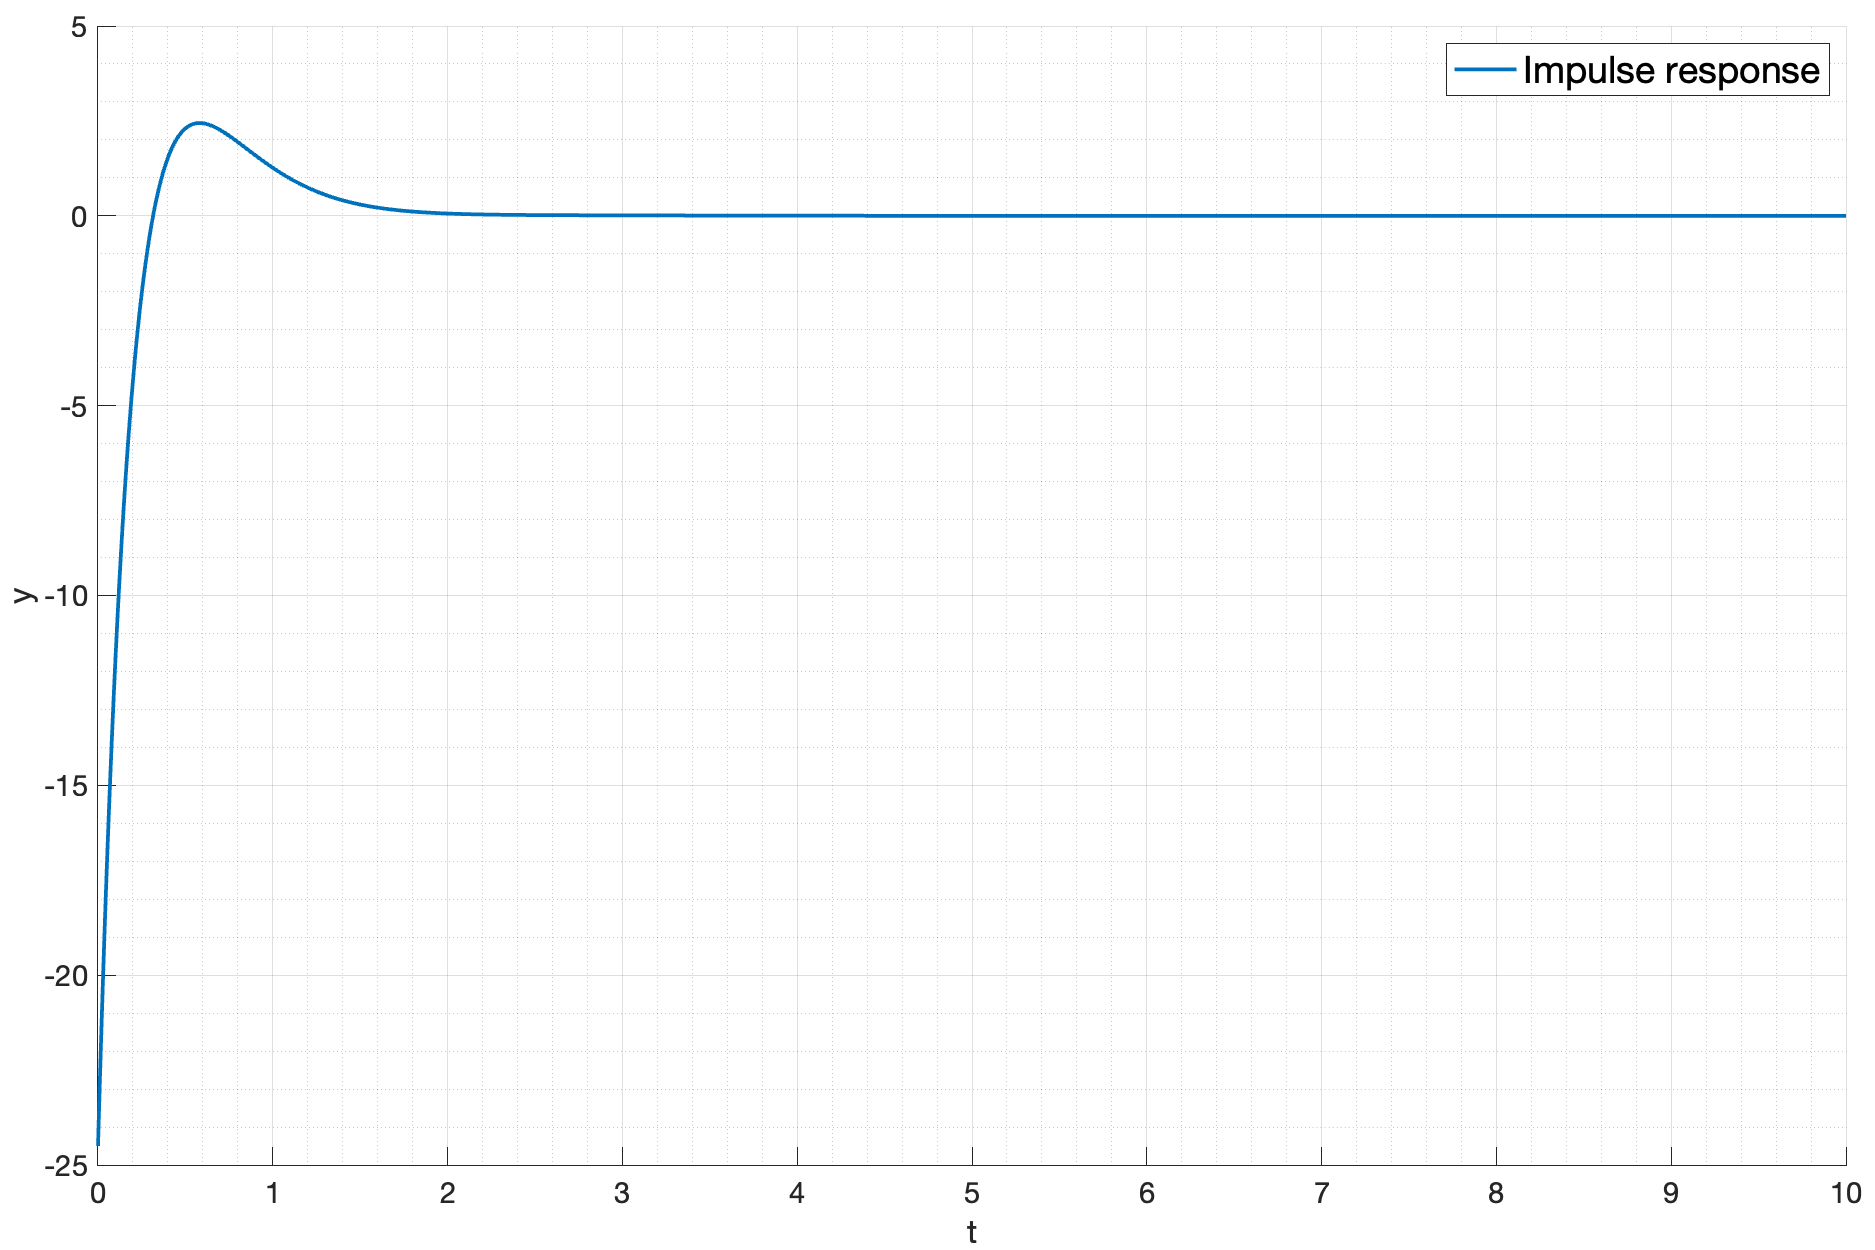
\includegraphics[width=\textwidth]{media/plots/task2_impulse_response_open.png}
        \caption{Замкнутая система (весовая)}
        \label{fig:task2_impulse:open}
    \end{subfigure}%
    \begin{subfigure}{0.5\textwidth}
        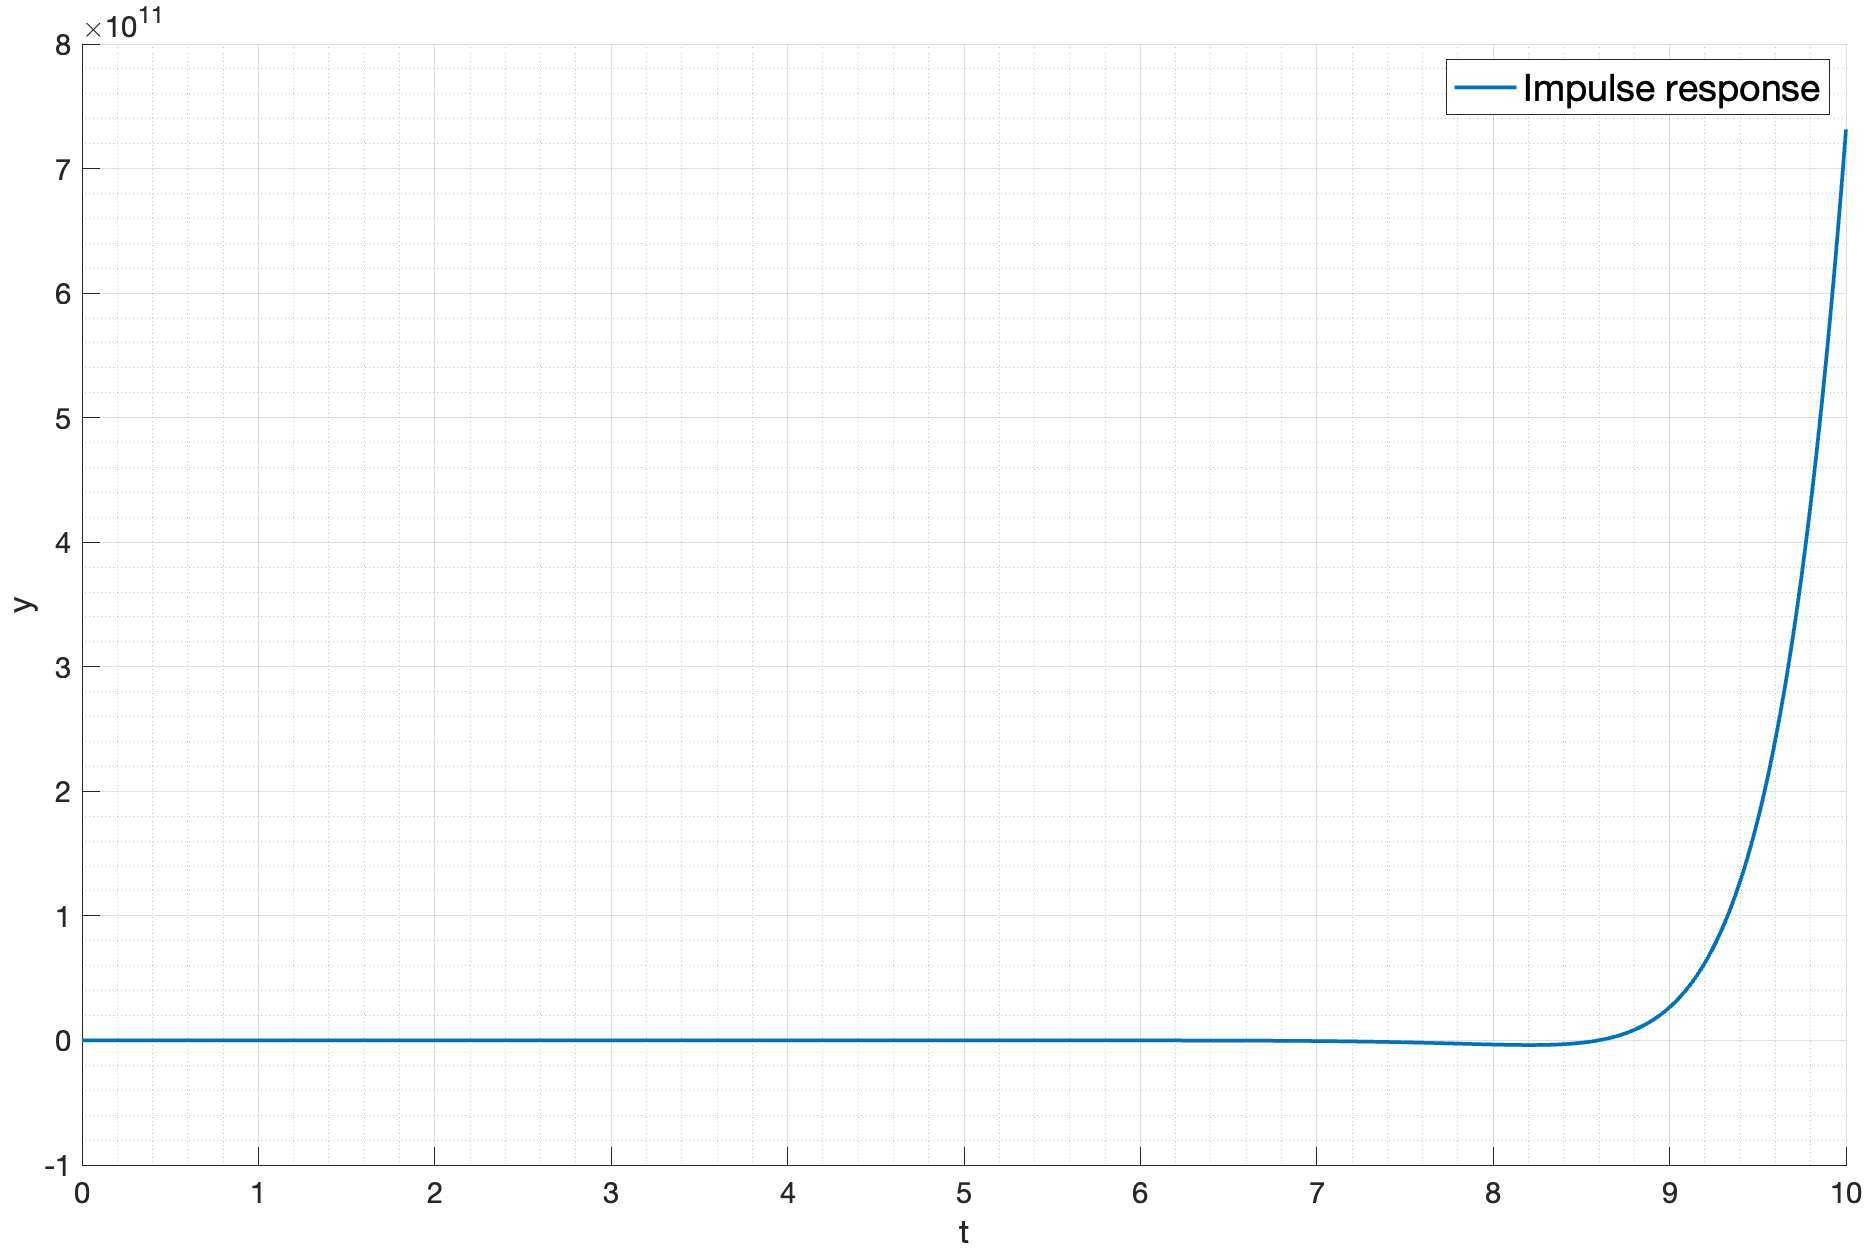
\includegraphics[width=\textwidth]{media/plots/task2_impulse_response_closed.png}
        \caption{Замкнутая система (весовая)}
        \label{fig:task2_impulse:closed}
    \end{subfigure}
    \caption{Переходные характеристики}
    \label{fig:task2_respoces}
\end{figure}

Годограф Найквиста приведен на рисунке \ref{fig:task2_nyquist}.
\begin{figure}[ht!]
    \centering
    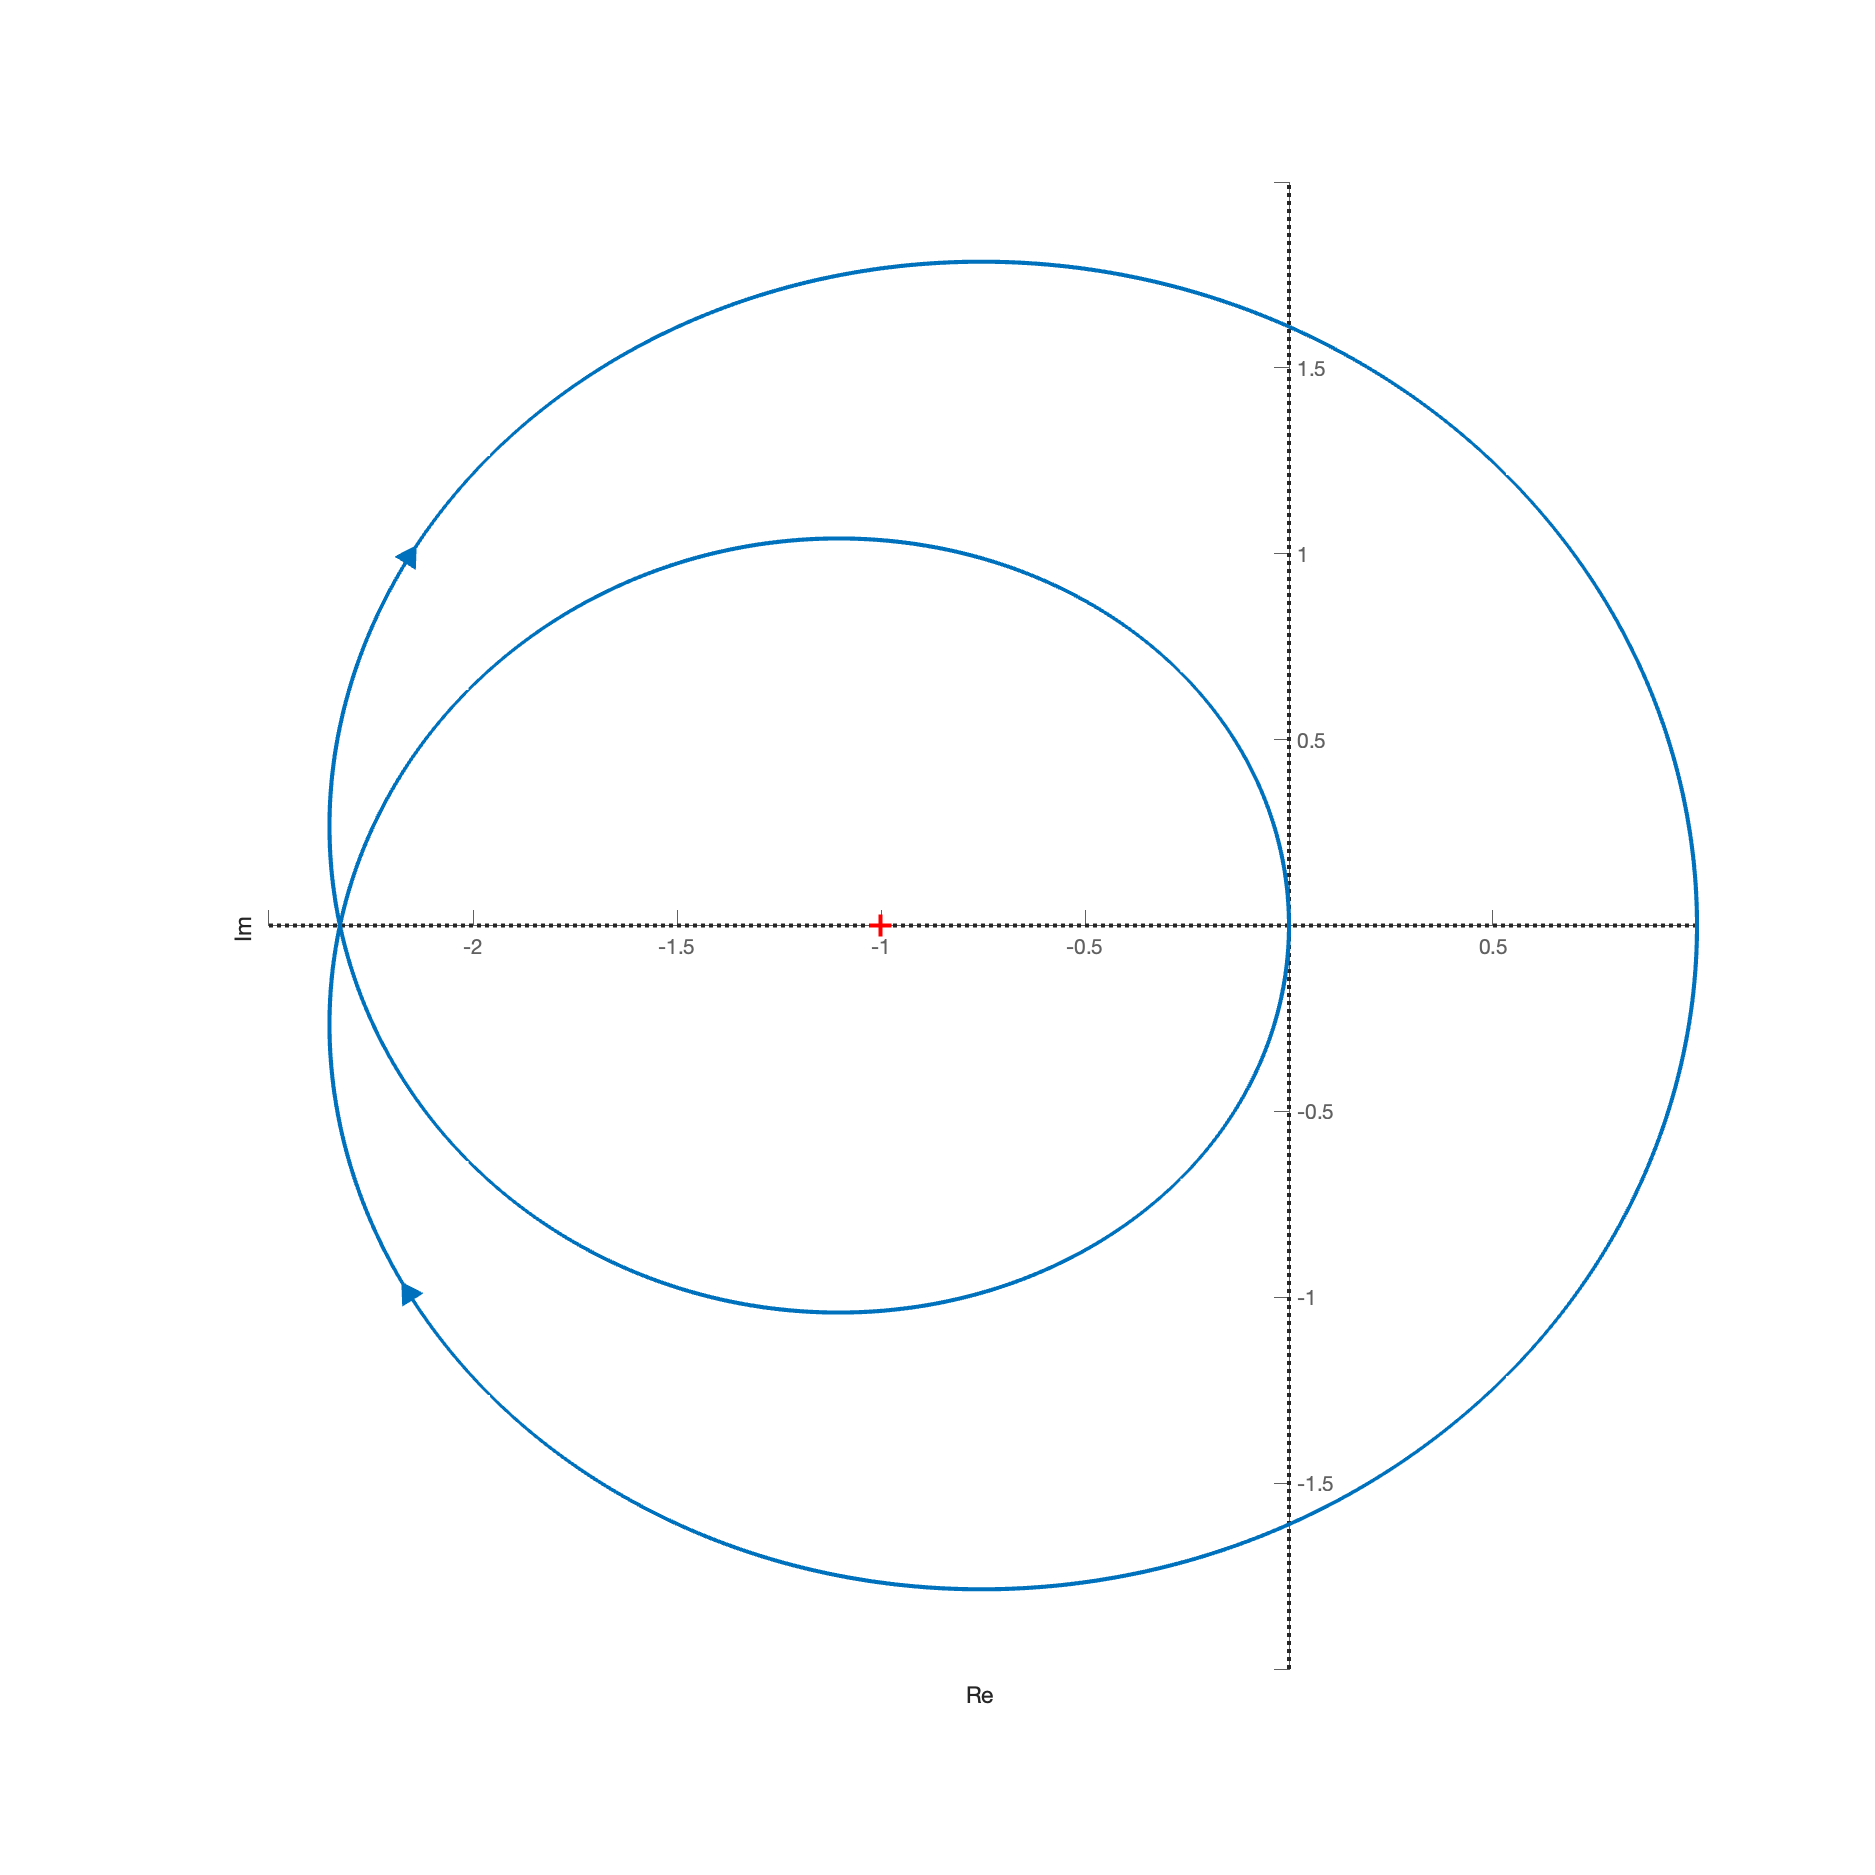
\includegraphics[width=\textwidth]{media/plots/task2_nyquist_open.png}
    \caption{Годограф Найквиста}
    \label{fig:task2_nyquist}
\end{figure}
Годограф делает 2 оборота вокруг точки $(-1, 0)$, количество неустойчивых полюсов замкнутой системы -- 0,
количество неустойчивых полюсов разомкнутой системы -- 2, следовательно, $Z = 2$, что подтверждает график на рисунке \ref{fig:task2_nyquist}.

Проведем анализ устойчивости на основе логарифмического критерий Найквиста, построим ЛАФЧХ разомкнутой системы (см. рис. \ref{fig:task2_bode_open}).
\begin{figure}[ht!]
    \centering
    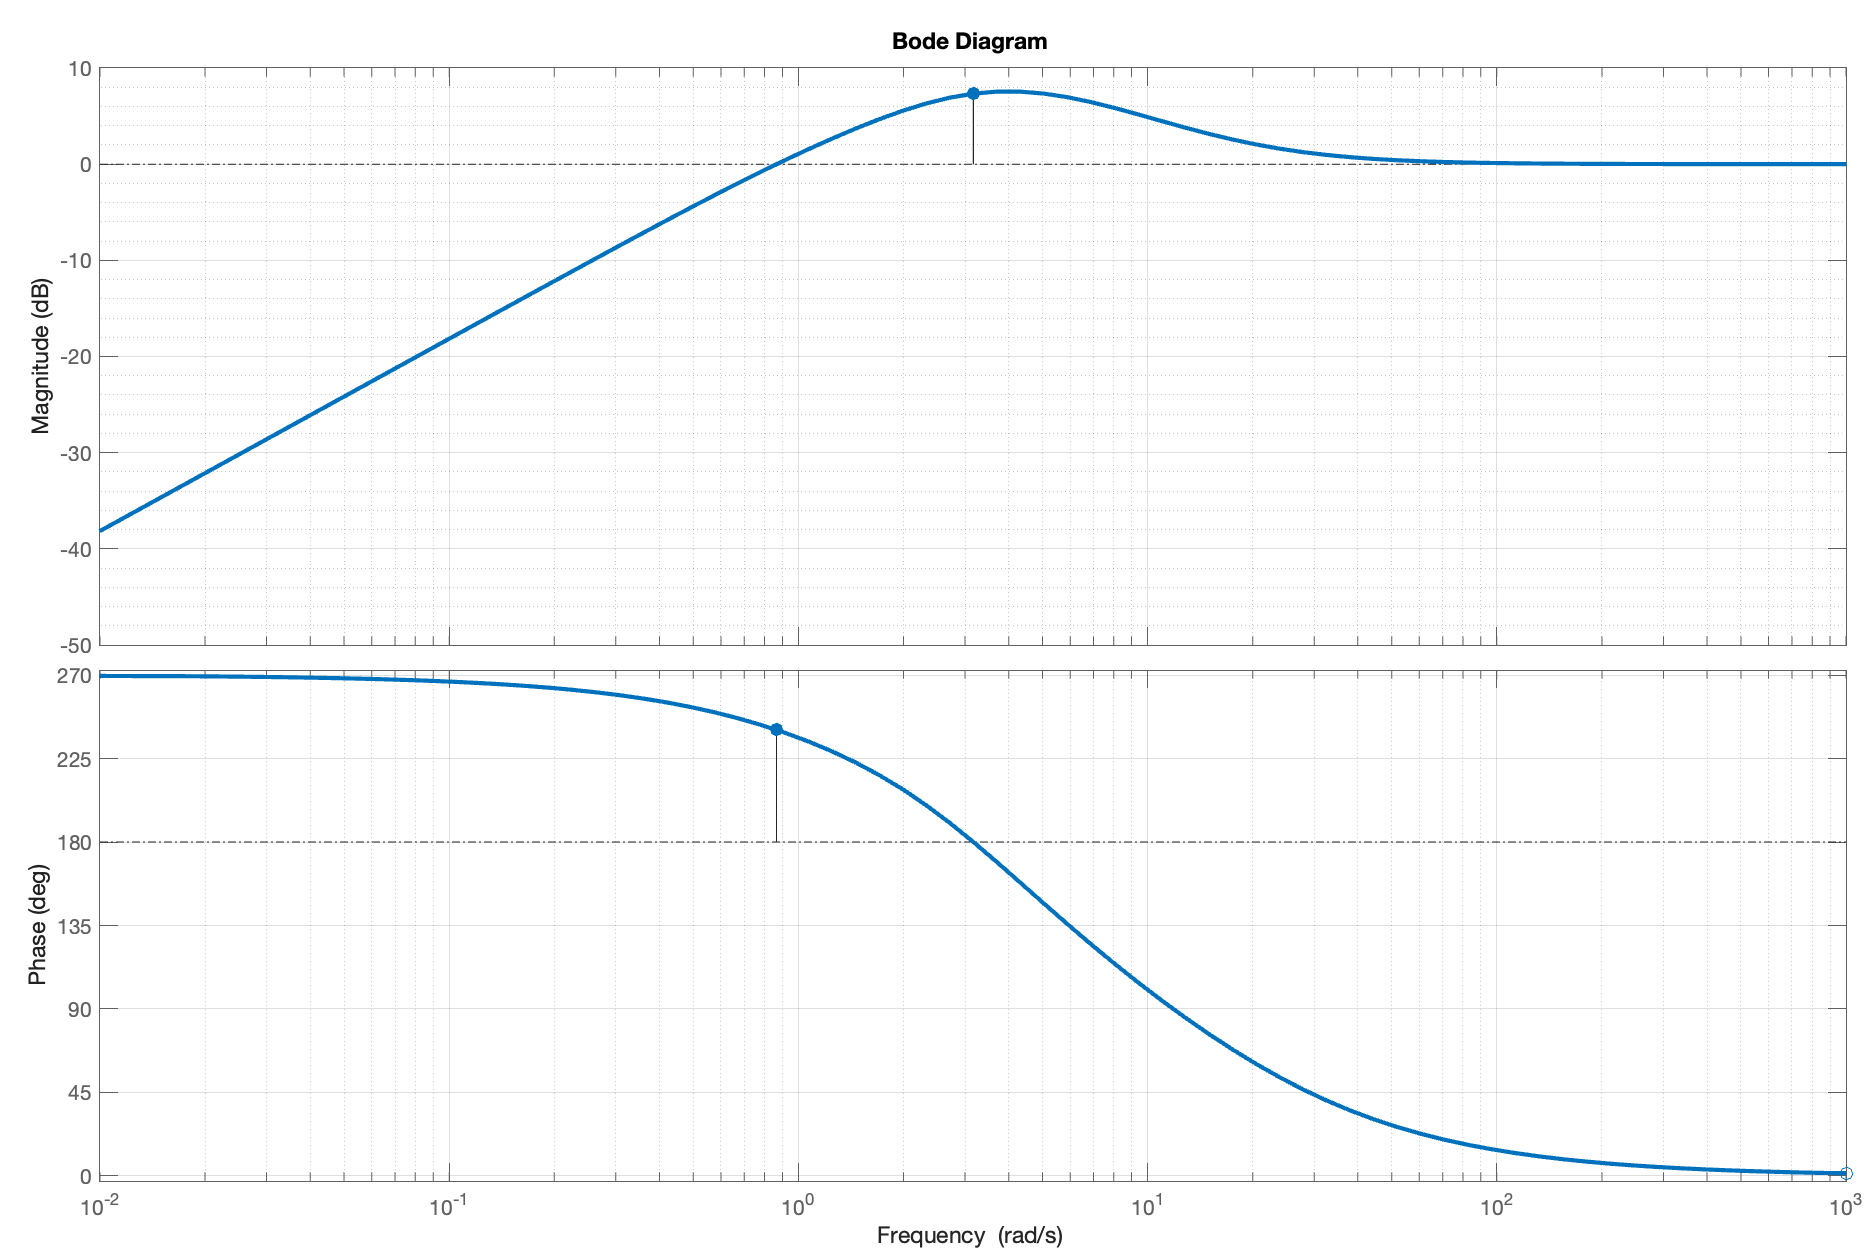
\includegraphics[width=\textwidth]{media/plots/task2_bode_open.png}
    \caption{ЛАФЧХ разомкнутой системы}
    \label{fig:task2_bode_open}
\end{figure}

Так как разомкнутая система имела 0 неустойчивых полюсов, нужно, чтобы число переходов через критические точки было равно 0.
На графике же видим один отрицательный переход через критическую точку, что подтверждает неустойчивость системы.

\FloatBarrier
\subsection{Система 3}
Зададимся системой с полюсами $P$:
\begin{equation}
    P = \begin{bmatrix}
        -1 & -1.5 & 2.5 & 3 & 3.5
    \end{bmatrix}
\end{equation}
И полюсами замкнутой системы $K$:
\begin{equation}
    K = \begin{bmatrix}
        -1 & -1.5 & -2.5 & -3 & -3.5
    \end{bmatrix}
\end{equation}

Запишем передаточные функции разомкнутой и замкнутой системы:
\begin{equation}
    W_{\text{o}} = \frac{s^5 +18.00s^4 +45.00s^3 +79.50s^2 +131.25s +78.75}{s^5 -6.50s^4 +5.75s^3 +27.12s^2 -25.50s -39.38}
\end{equation}
\begin{equation}
    W_{\text{c}} = \frac{s^5 +18.00s^4 +45.00s^3 +79.50s^2 +131.25s +78.75}{2s^5 +11.50s^4 +50.75s^3 +106.62s^2 +105.75s +39.38}
\end{equation}

Карты расположения полюсов передаточных функций приведены на рисунках \ref{fig:task3_poles:open} и \ref{fig:task3_poles:closed} соответственно.
\begin{figure}
    \centering
    \begin{subfigure}{0.5\textwidth}
        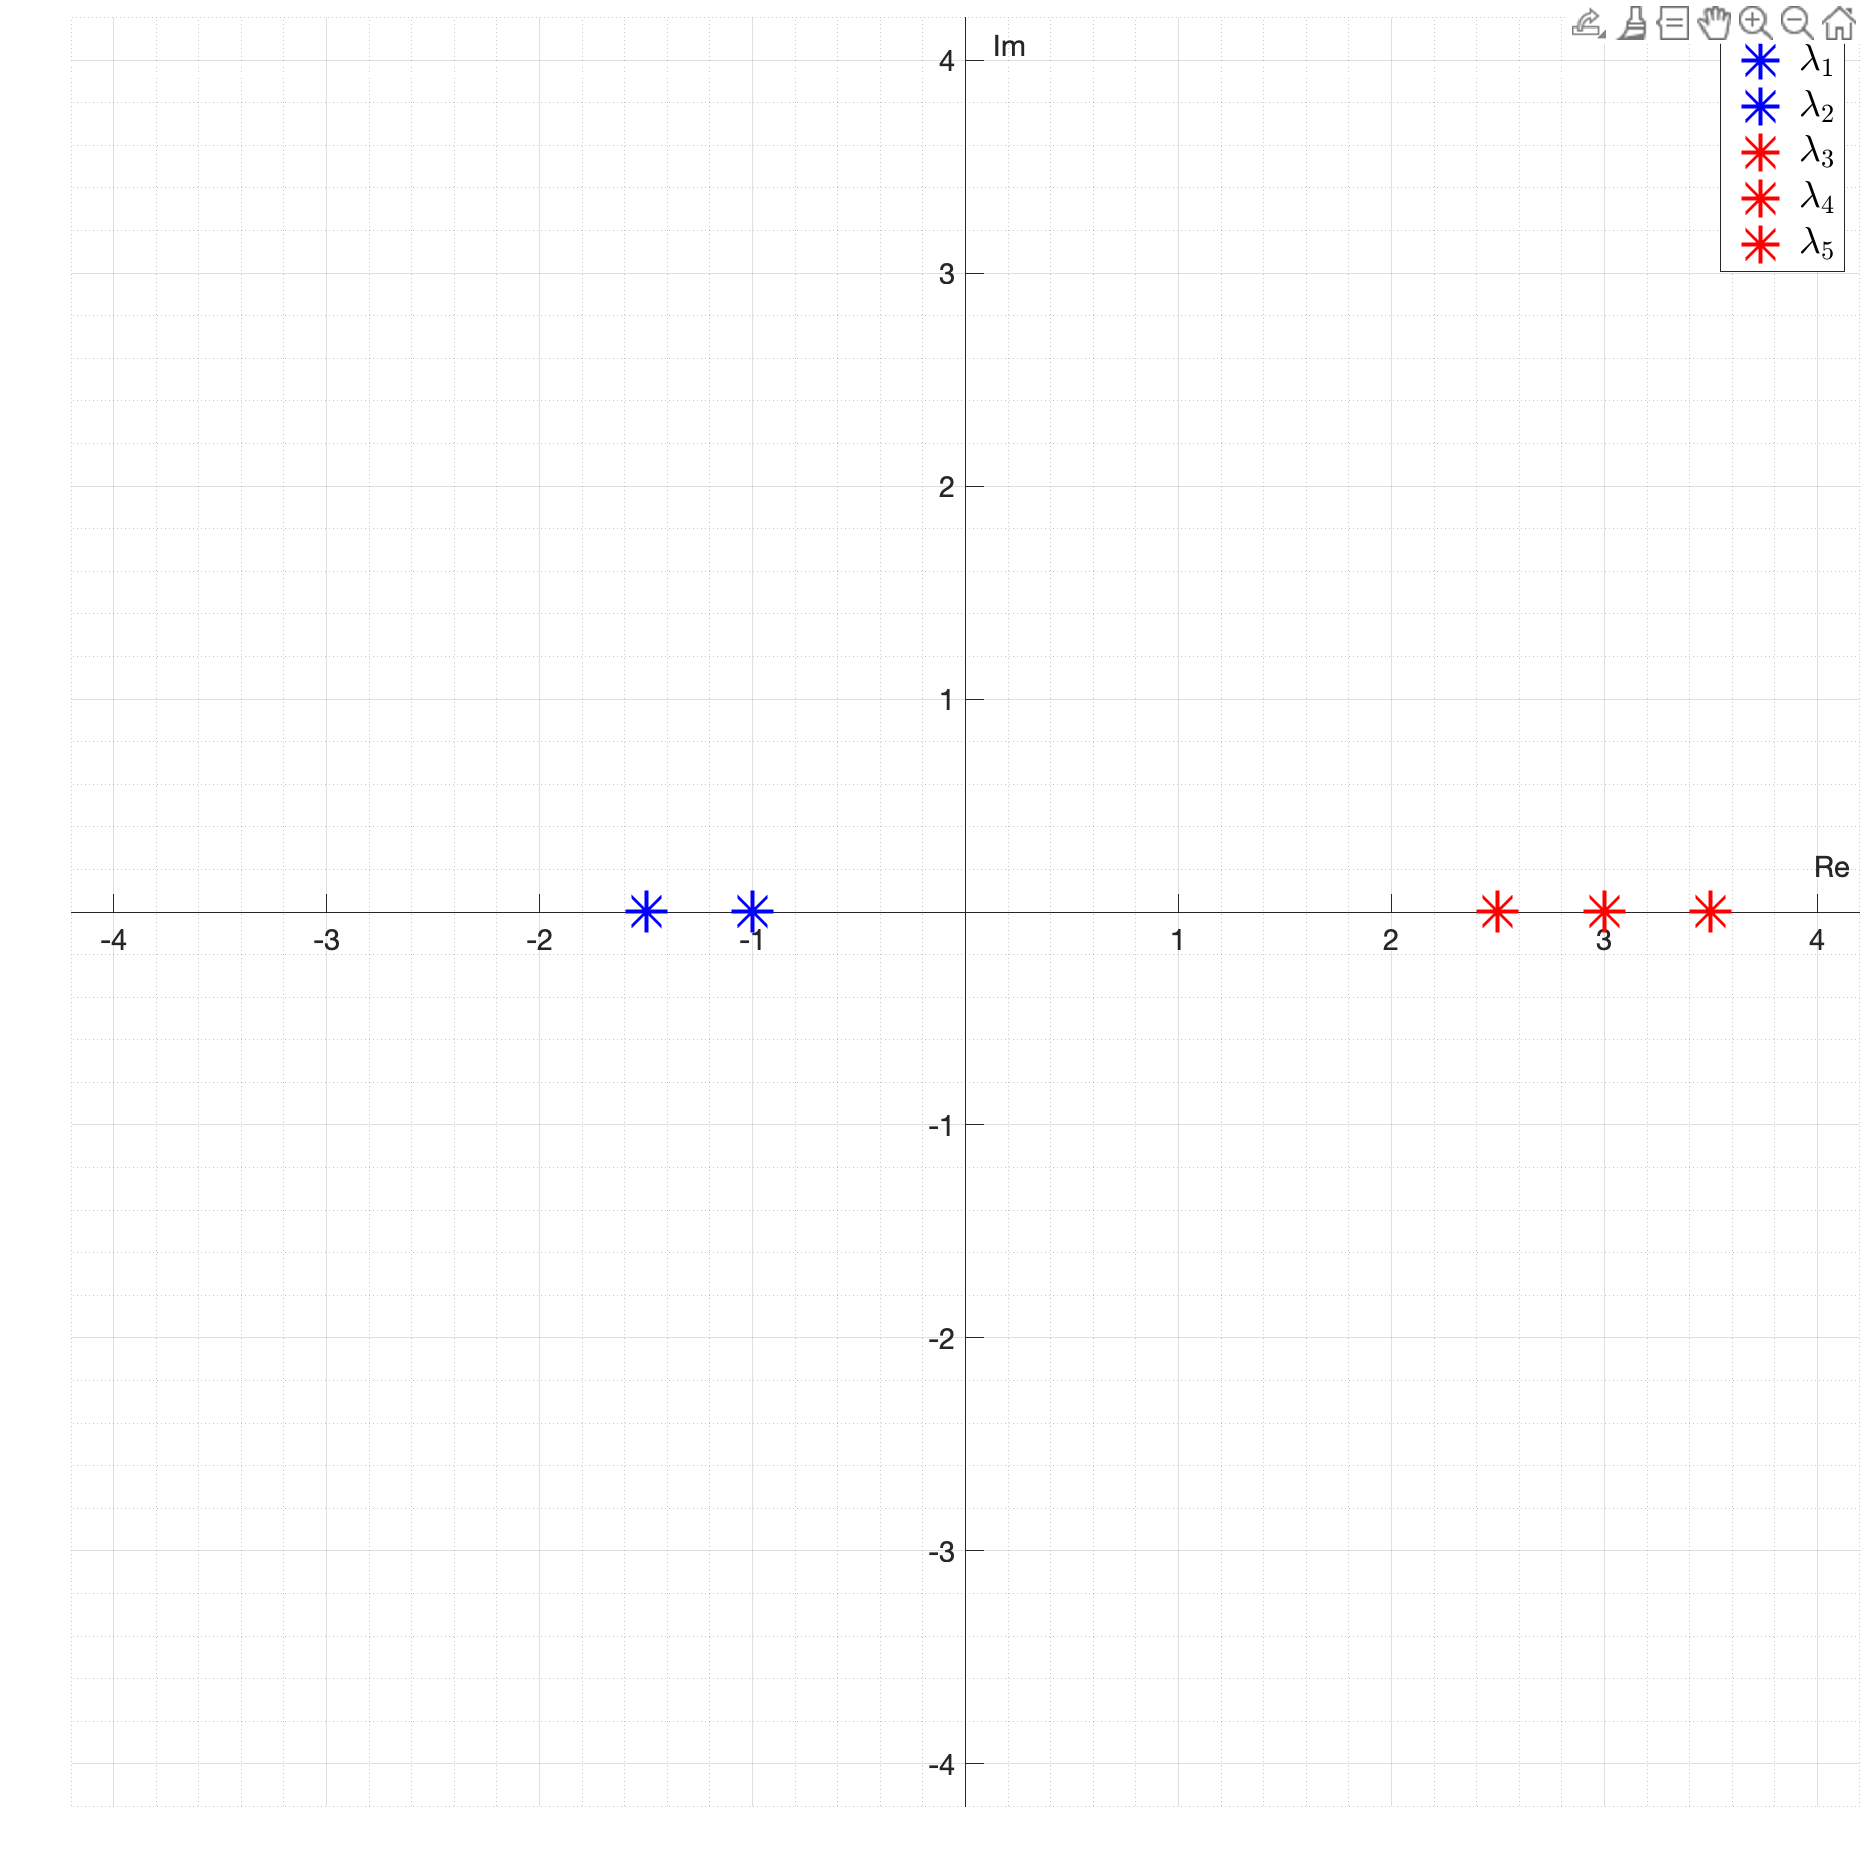
\includegraphics[width=\textwidth]{media/plots/task3_poles_open.png}
        \caption{Разомкнутая система}
        \label{fig:task3_poles:open}
    \end{subfigure}%
    \begin{subfigure}{0.5\textwidth}
        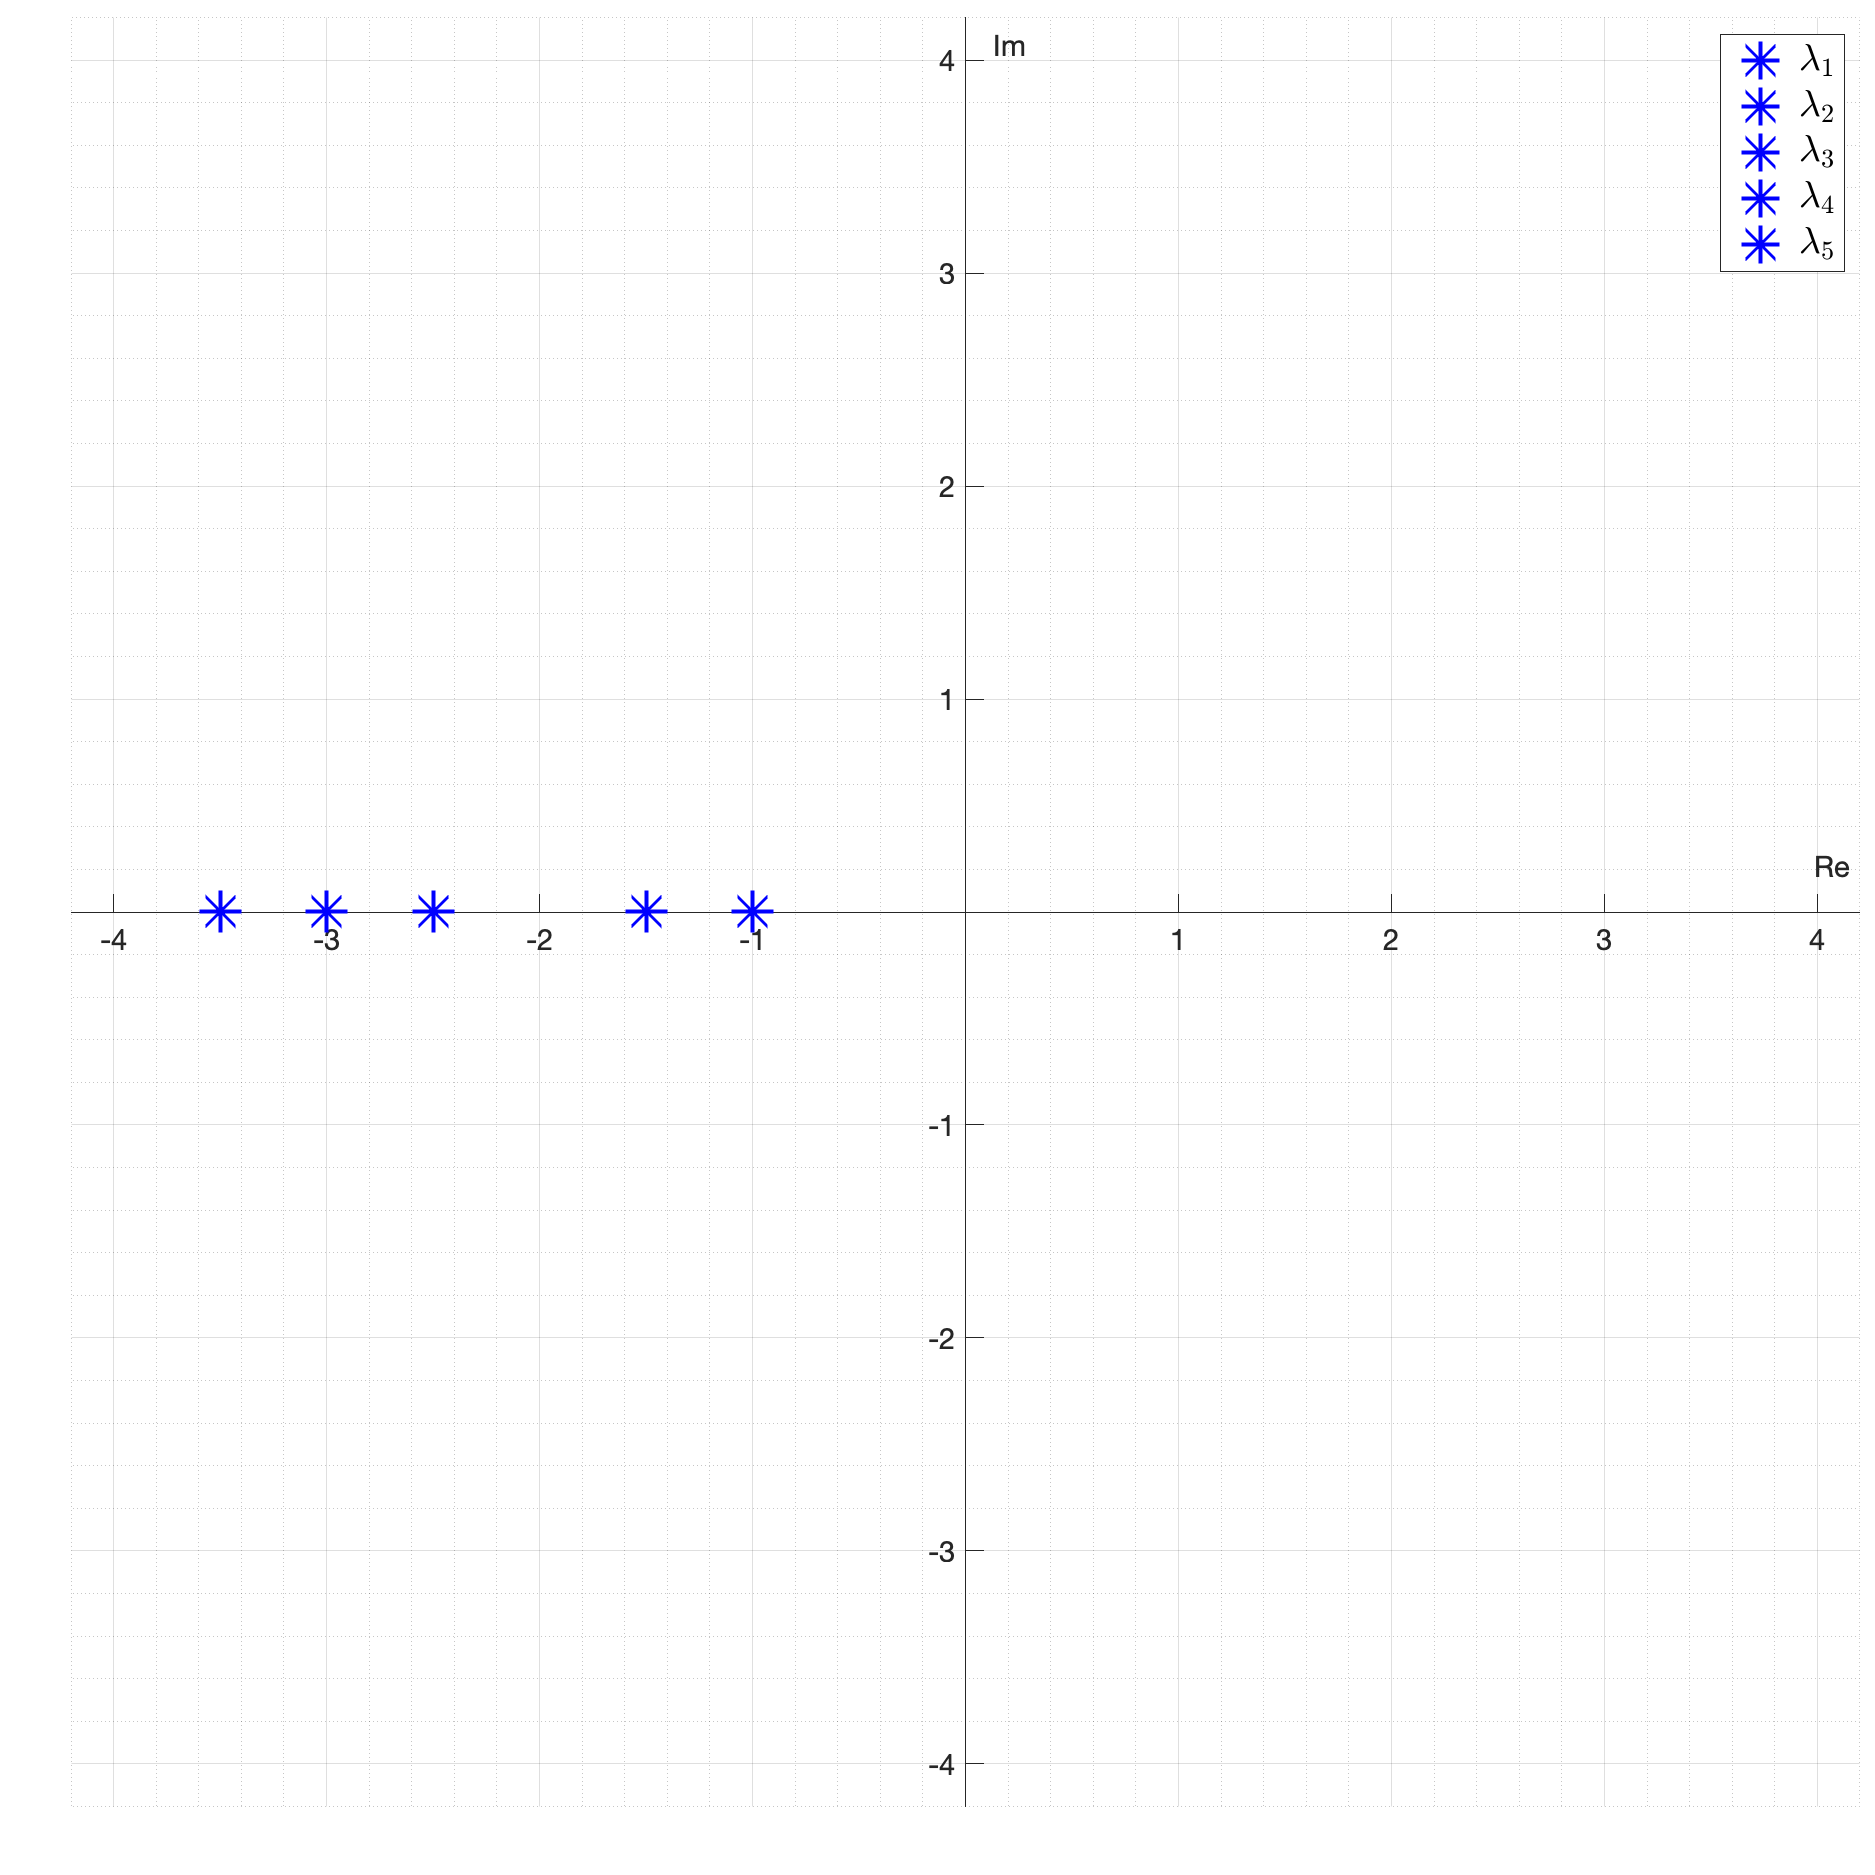
\includegraphics[width=\textwidth]{media/plots/task3_poles_closed.png}
        \caption{Замкнутая система}
        \label{fig:task3_poles:closed}
    \end{subfigure}
    \caption{Карты расположения полюсов}
    \label{fig:task3_poles}
\end{figure}

Переходные характеристики систем приведены на рисунке \ref{fig:task3_respoces}.
\begin{figure}[ht!]
    \centering
    \begin{subfigure}{0.5\textwidth}
        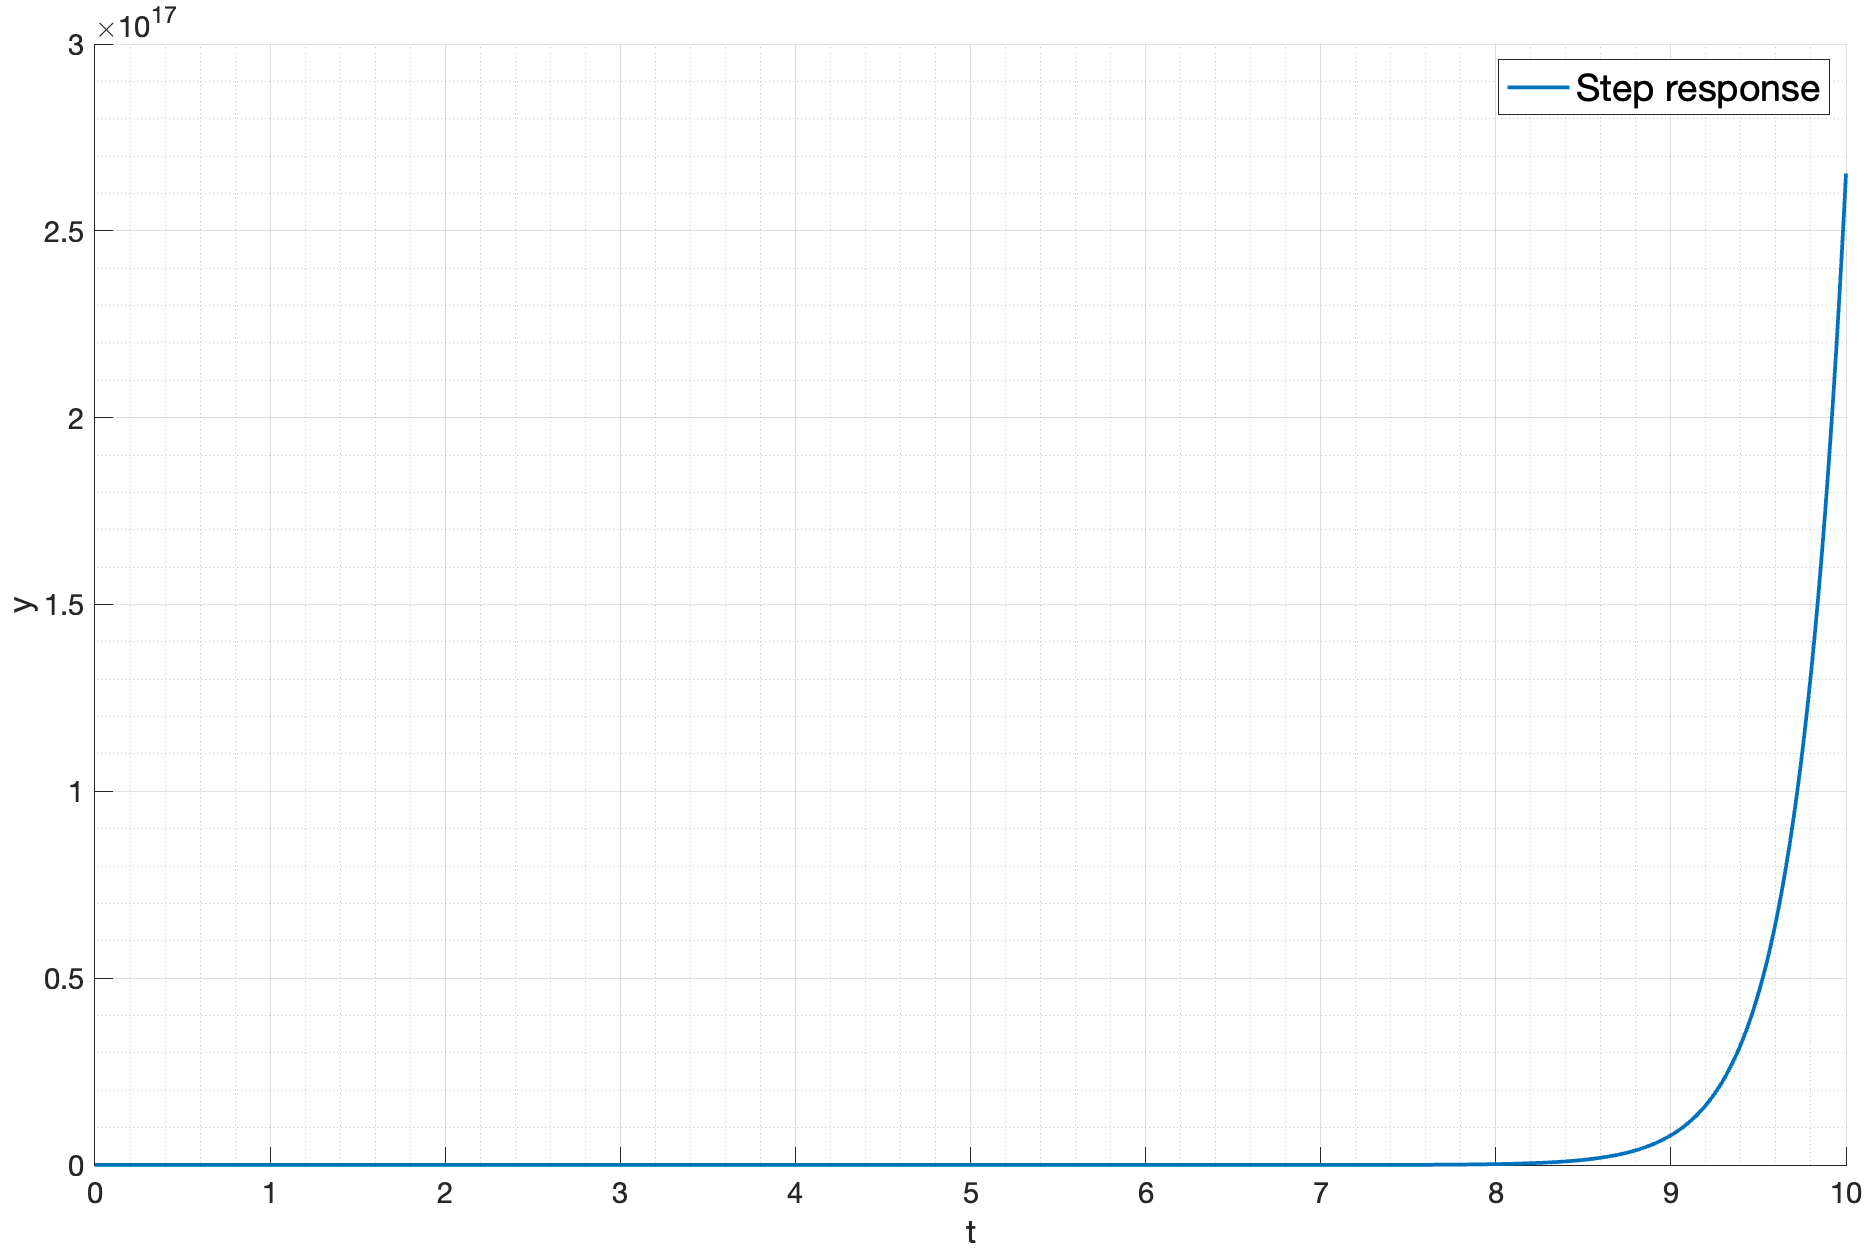
\includegraphics[width=\textwidth]{media/plots/task3_step_response_open.png}
        \caption{Разомкнутая система (переходная)}
        \label{fig:task3_step:open}
    \end{subfigure}%
    \begin{subfigure}{0.5\textwidth}
        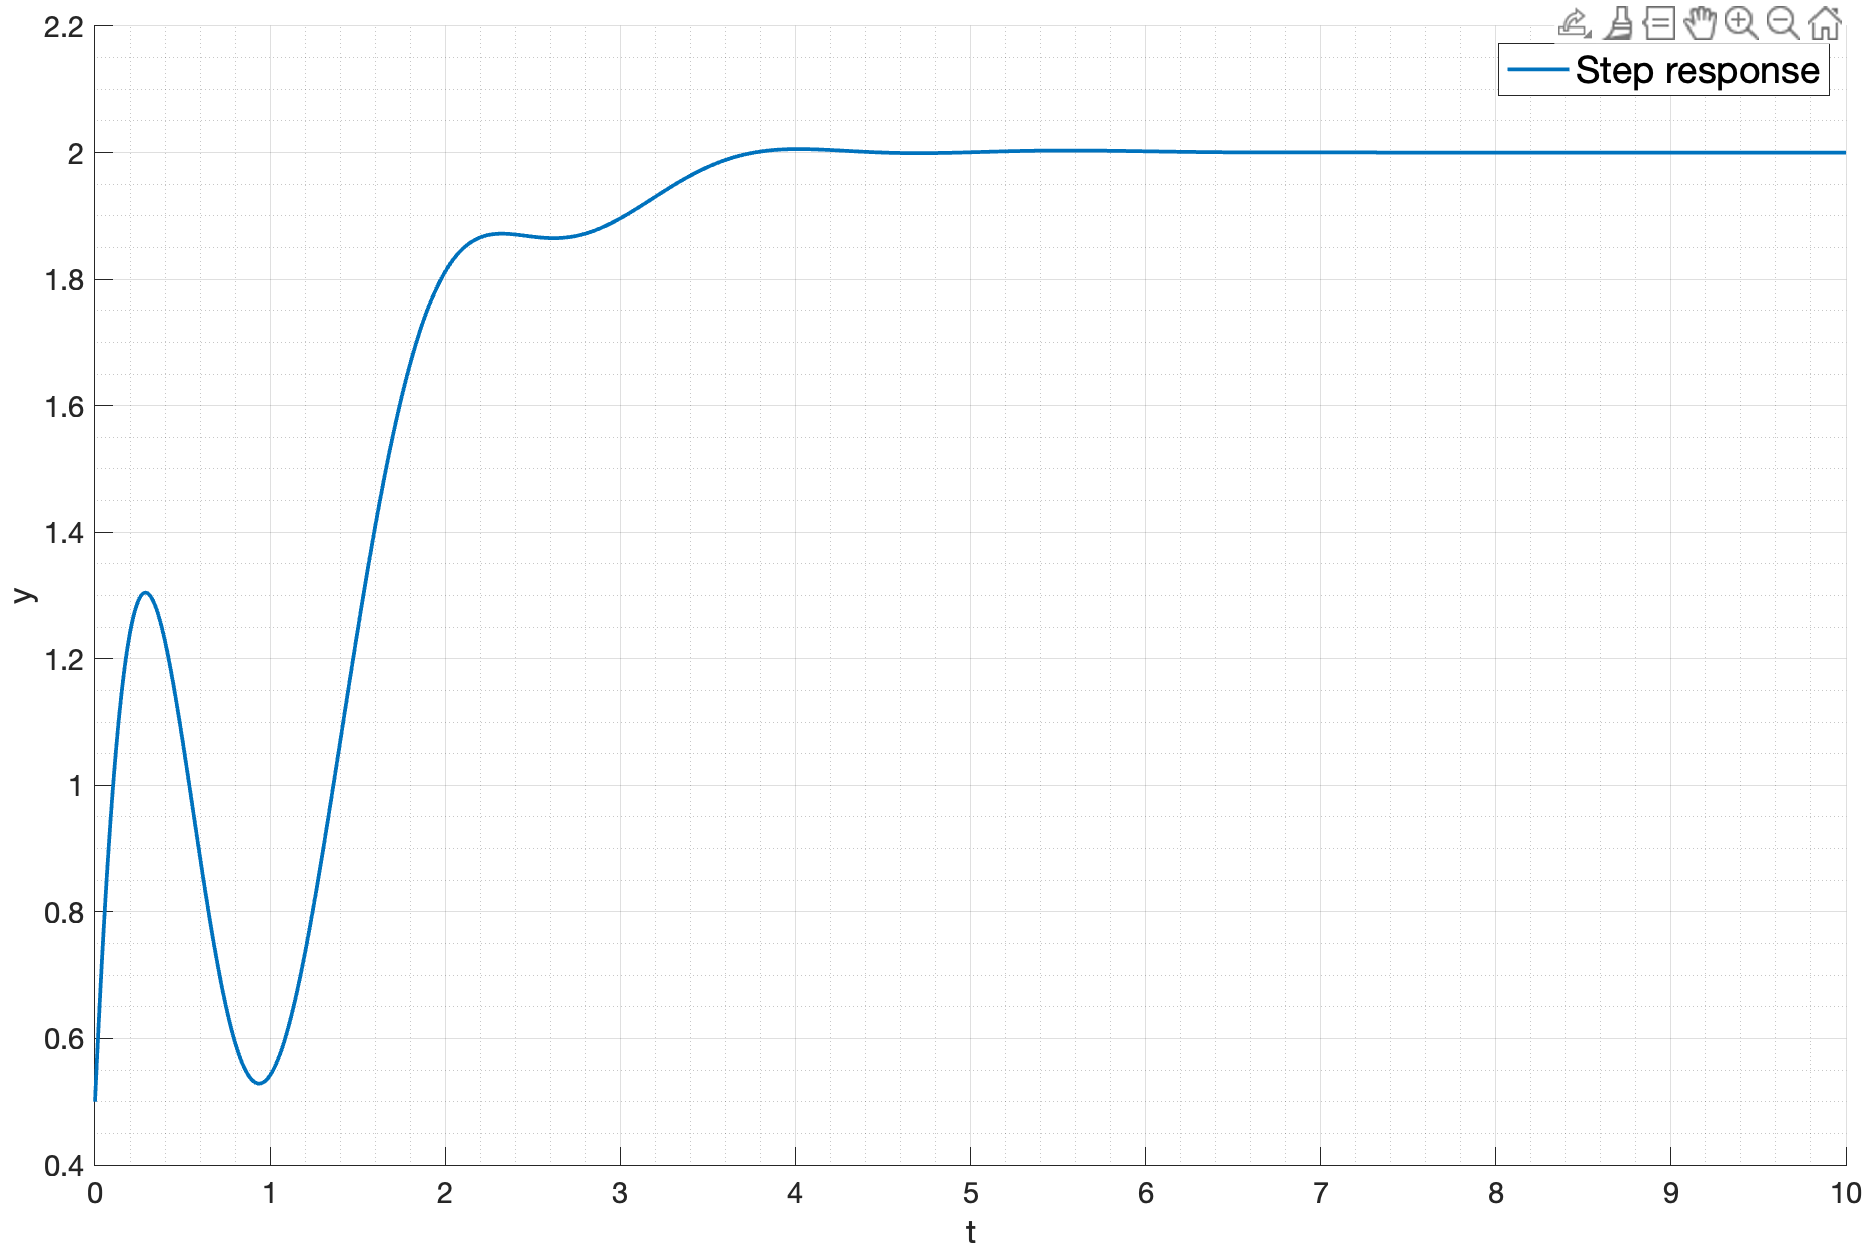
\includegraphics[width=\textwidth]{media/plots/task3_step_response_closed.png}
        \caption{Замкнутая система (переходная)}
        \label{fig:task3_step:closed}
    \end{subfigure}
    \begin{subfigure}{0.5\textwidth}
        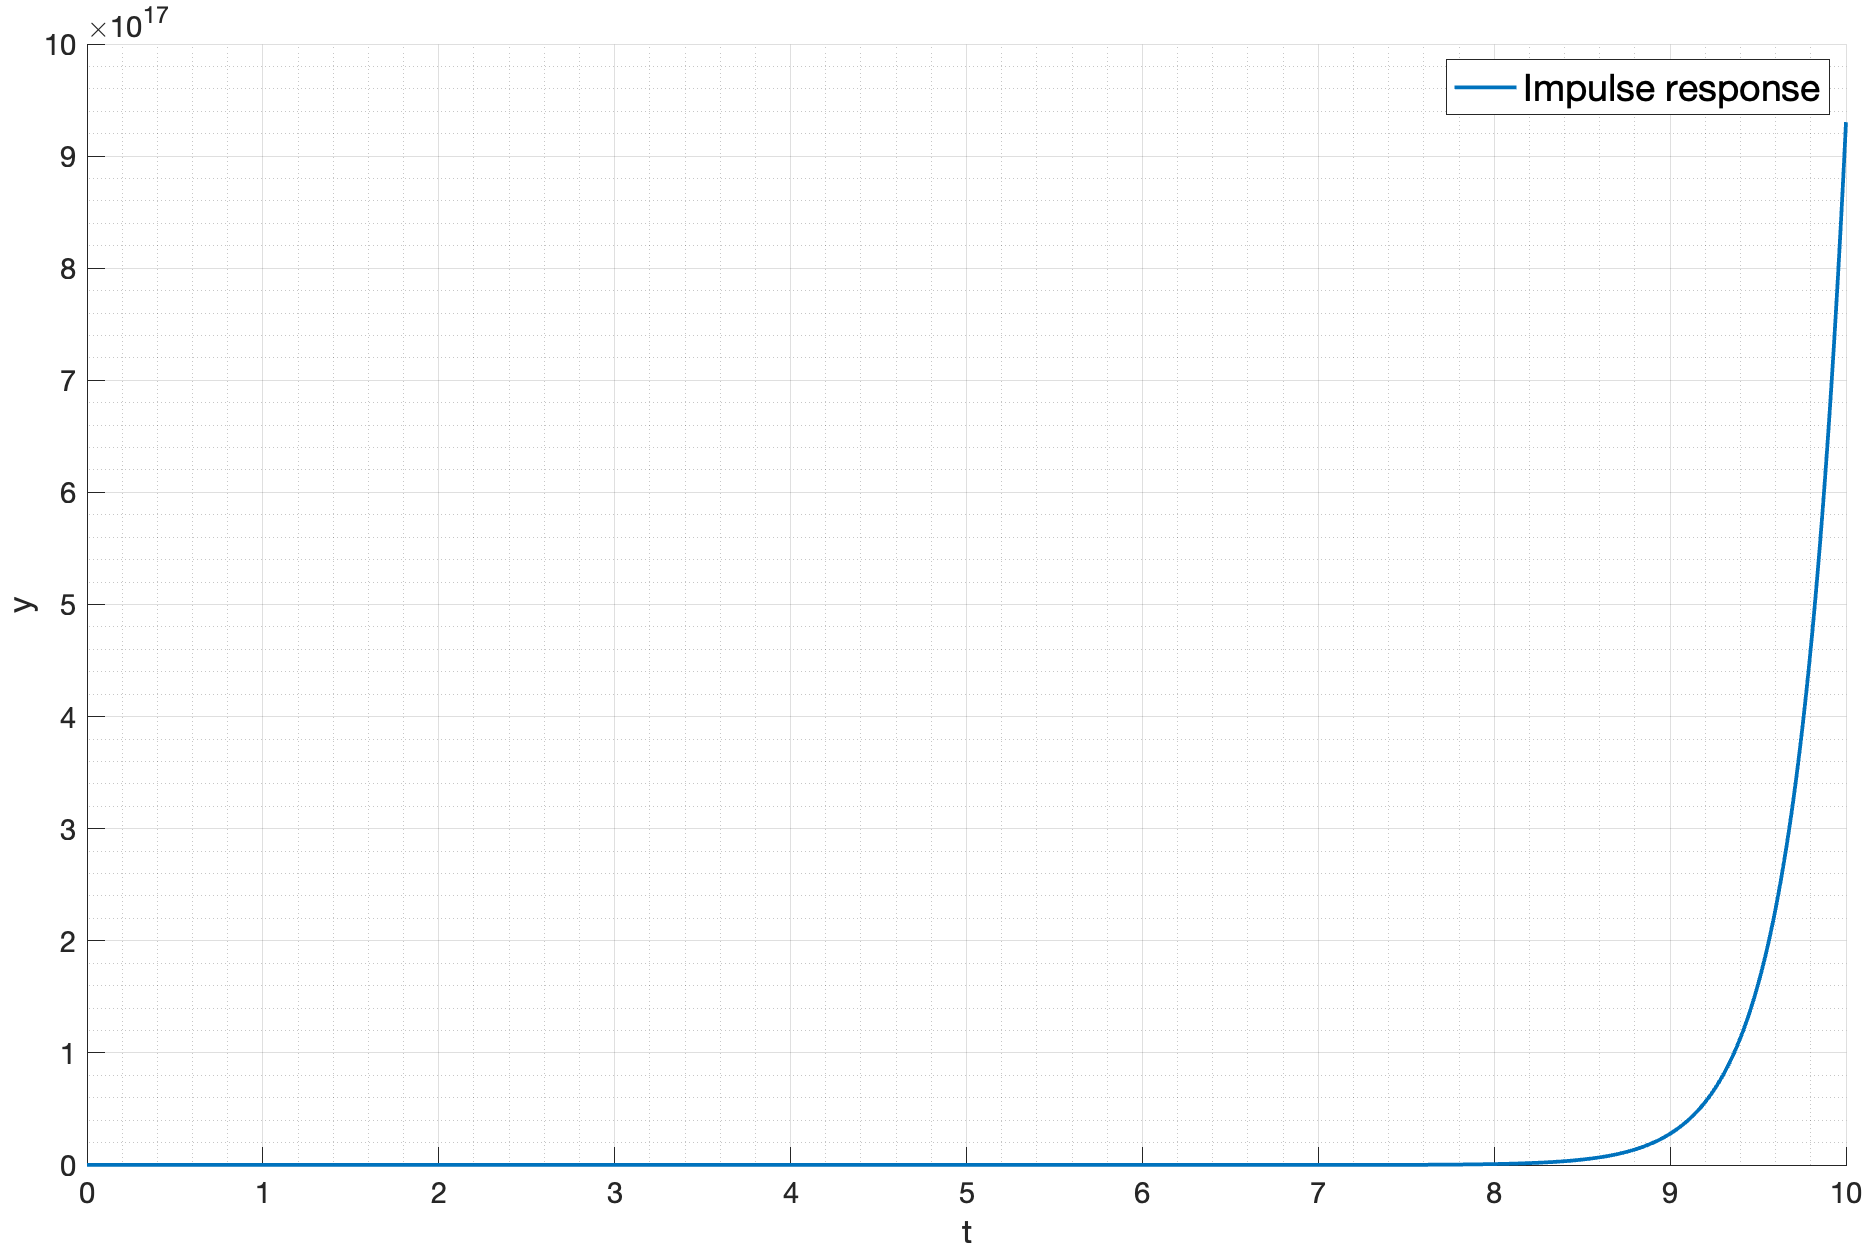
\includegraphics[width=\textwidth]{media/plots/task3_impulse_response_open.png}
        \caption{Замкнутая система (весовая)}
        \label{fig:task3_impulse:open}
    \end{subfigure}%
    \begin{subfigure}{0.5\textwidth}
        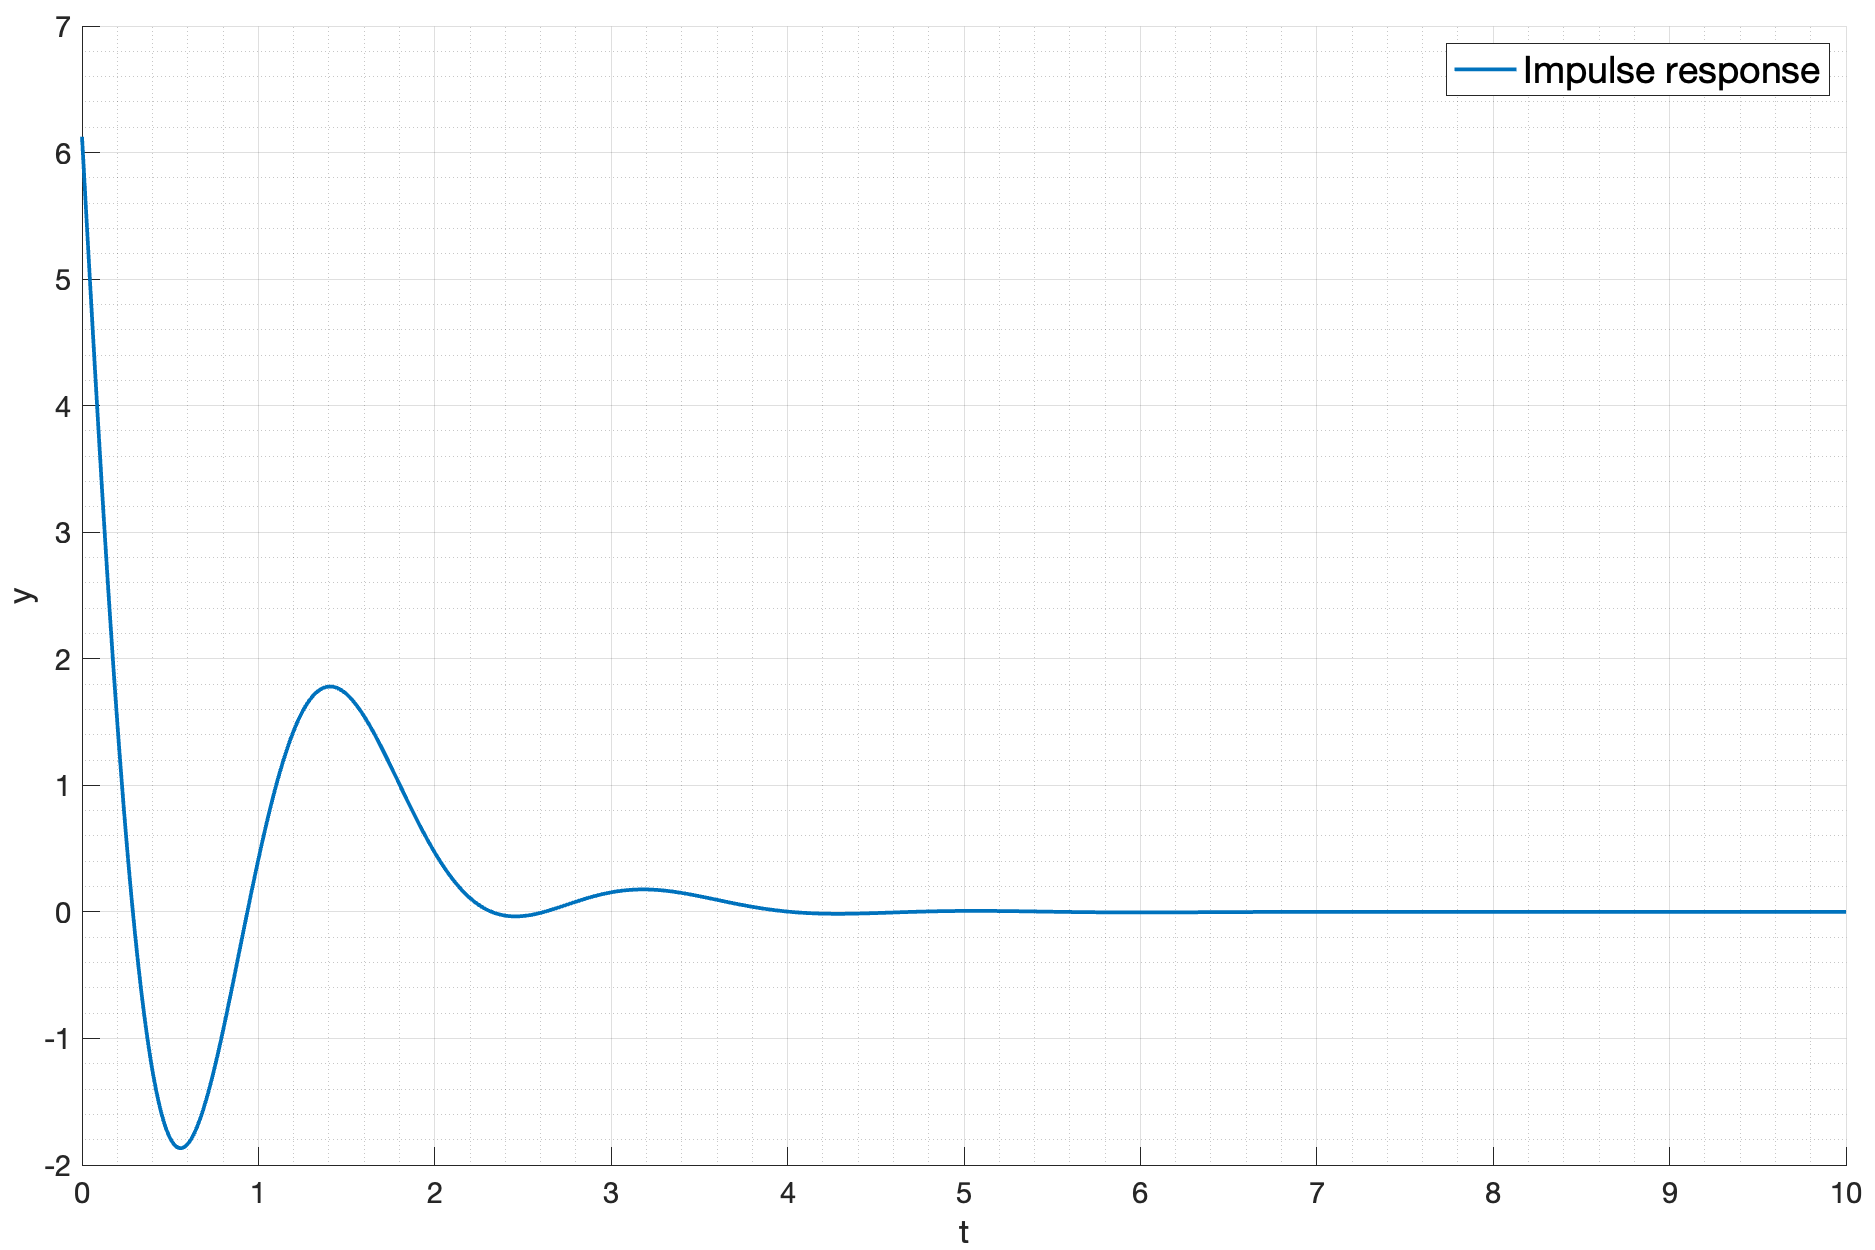
\includegraphics[width=\textwidth]{media/plots/task3_impulse_response_closed.png}
        \caption{Замкнутая система (весовая)}
        \label{fig:task3_impulse:closed}
    \end{subfigure}
    \caption{Переходные характеристики}
    \label{fig:task3_respoces}
\end{figure}

Годограф Найквиста приведен на рисунке \ref{fig:task3_nyquist}.
\begin{figure}[ht!]
    \centering
    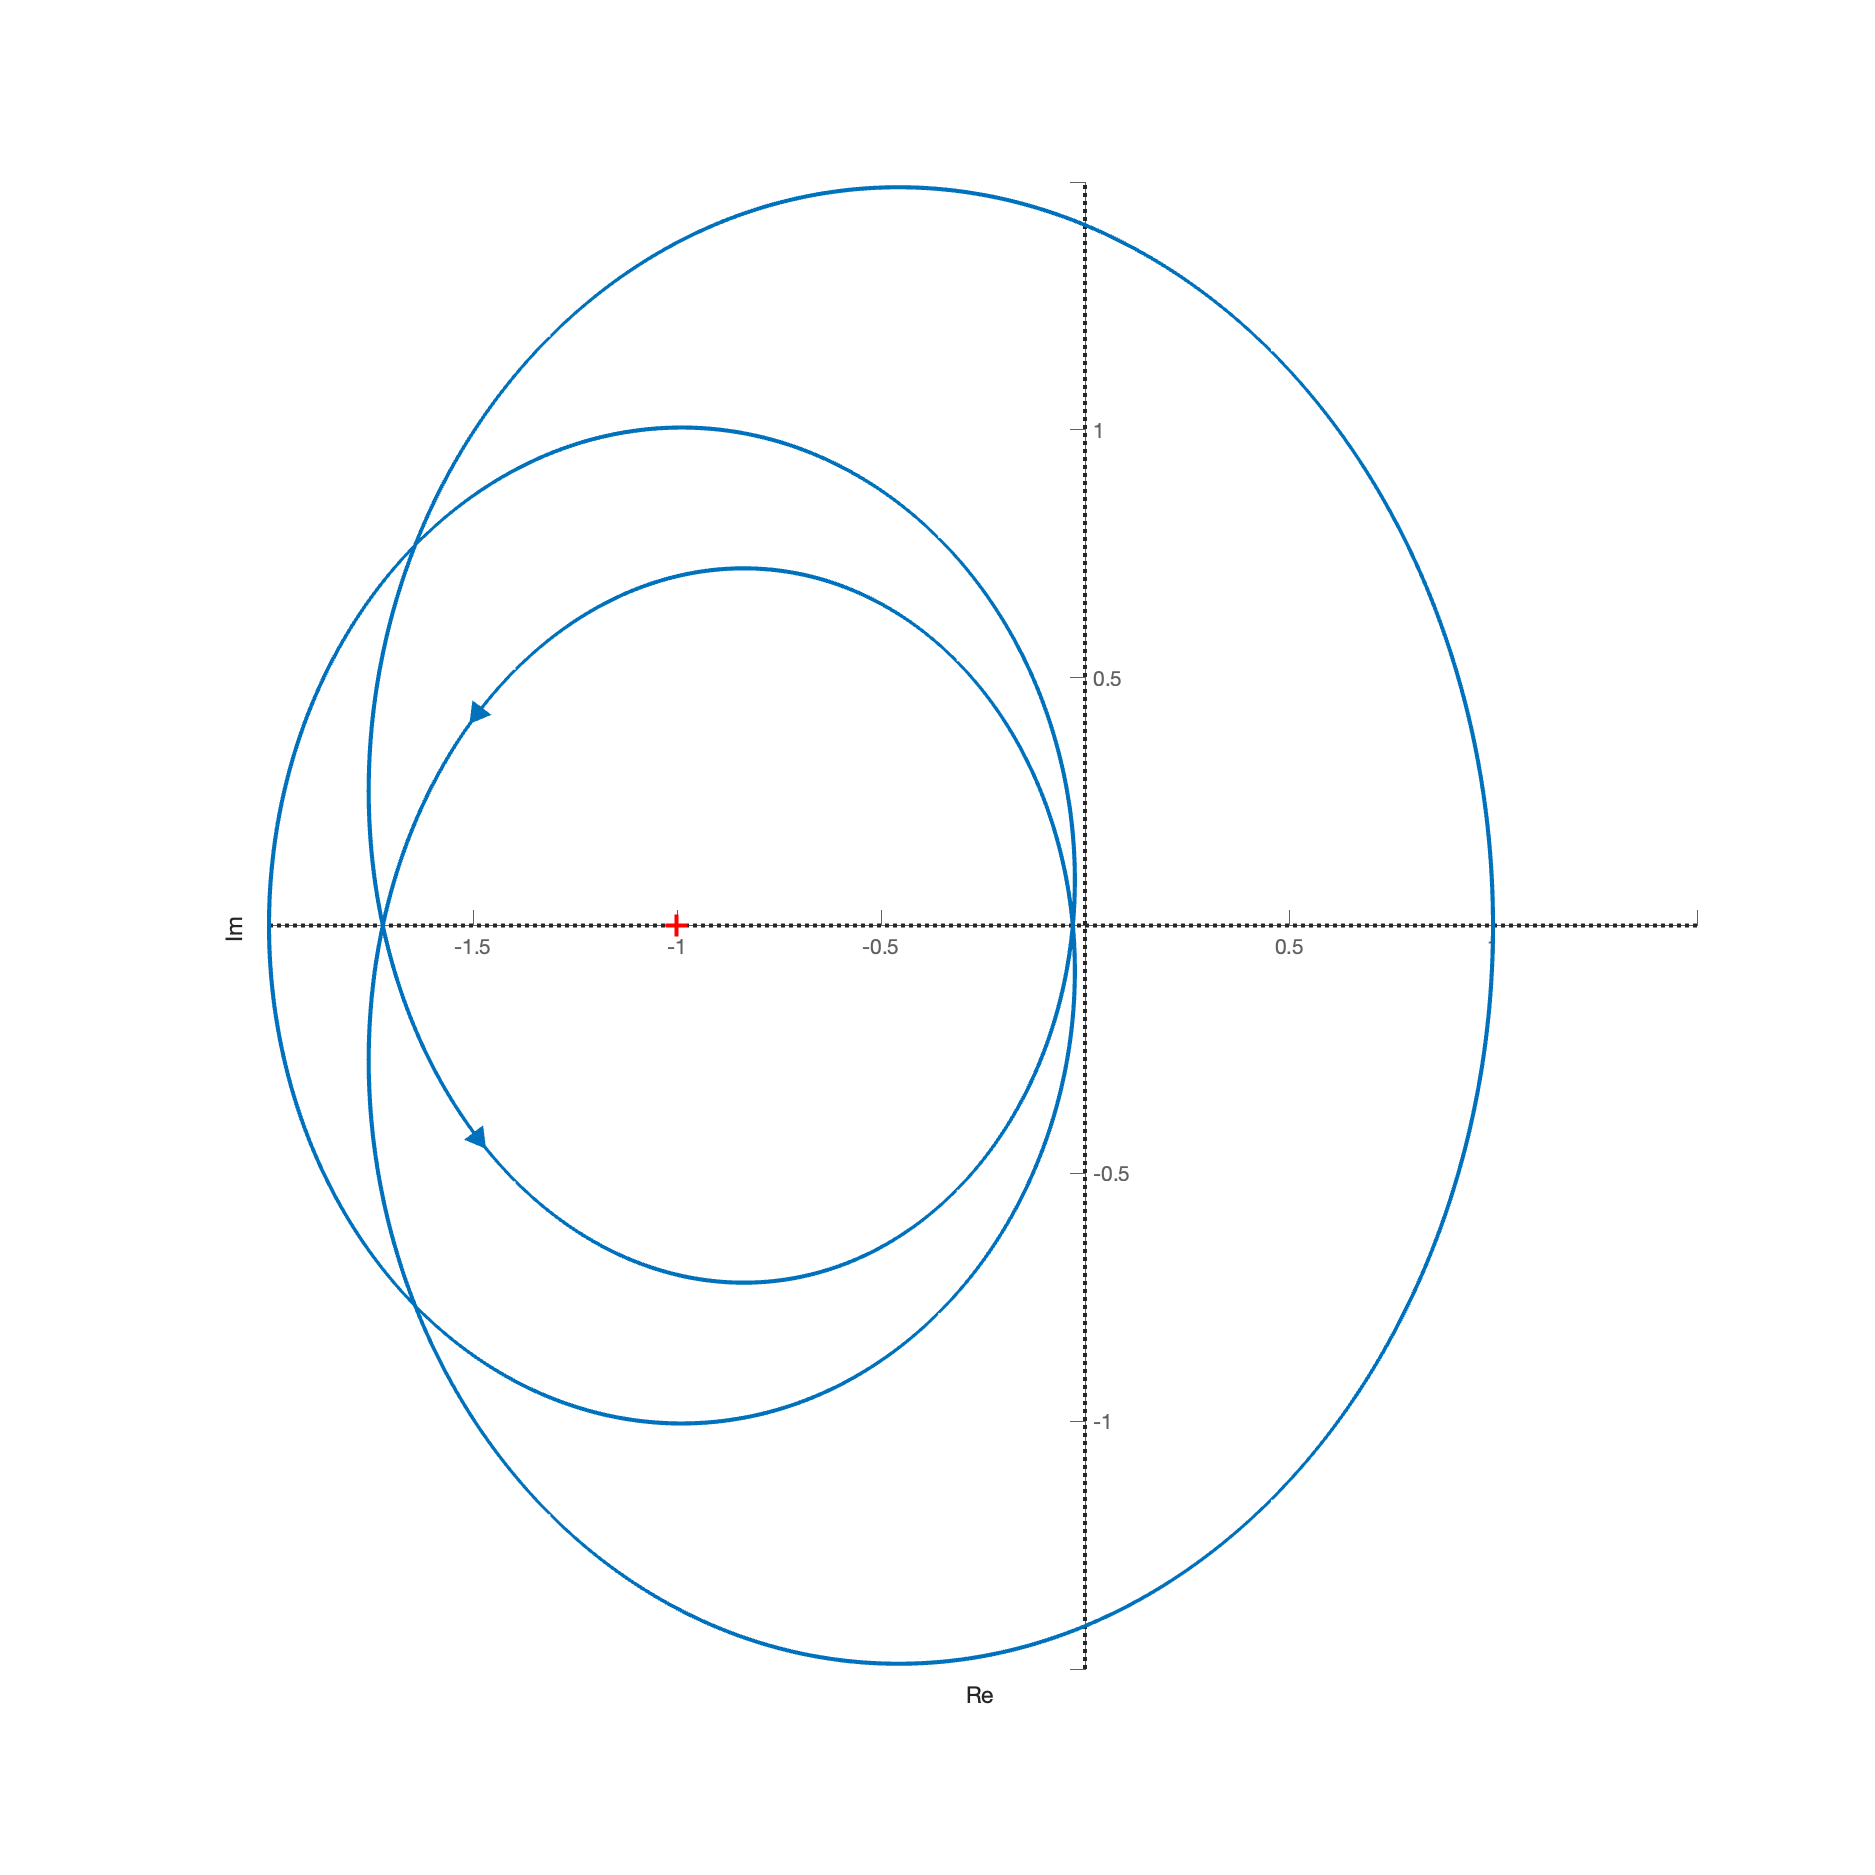
\includegraphics[width=\textwidth]{media/plots/task3_nyquist_open.png}
    \caption{Годограф Найквиста}
    \label{fig:task3_nyquist}
\end{figure}

Количество неустойчивых полюсов замкнутой системы -- 0, количество неустойчивых полюсов разомкнутой системы -- 3, следовательно, $Z = -3$, что подтверждает график на рисунке \ref{fig:task3_nyquist}.

Проведем анализ устойчивости на основе логарифмического критерий Найквиста, построим ЛАФЧХ разомкнутой системы (см. рис. \ref{fig:task3_bode_open}).
\begin{figure}[ht!]
    \centering
    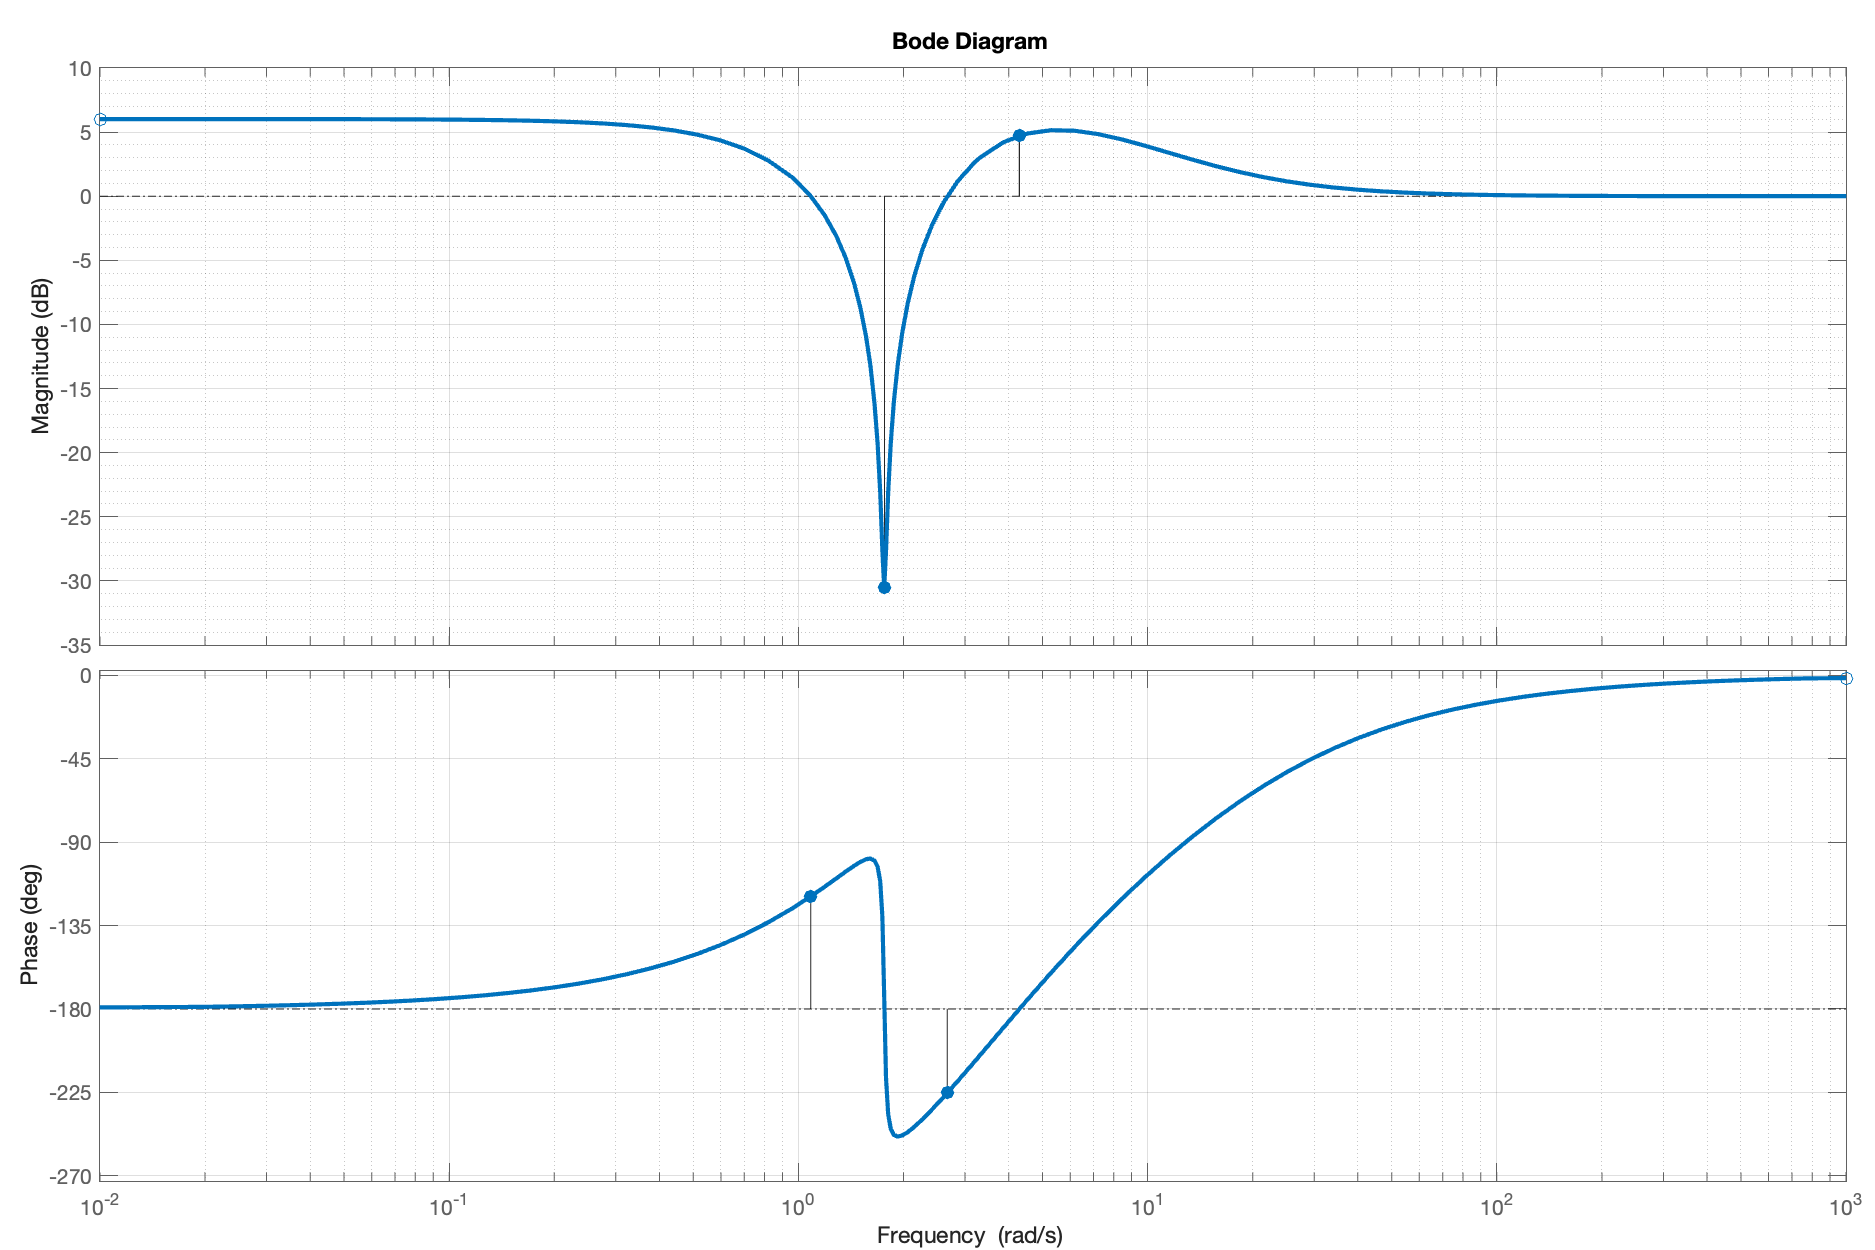
\includegraphics[width=\textwidth]{media/plots/task3_bode_open.png}
    \caption{ЛАФЧХ разомкнутой системы}
    \label{fig:task3_bode_open}
\end{figure}

Так как разомкнутая система имела 3 неустойчивых полюса, нужно, чтобы число переходов через критические точки было равно 1.5.
ЛАФЧХ начинается с критического отрезка и делает один положительный переход через критическую точку, что дает сумму переходов равную 1.5, что подтверждает устойчивость системы.

\subsection{Вывод}
Критерий Найквиста позволяет оценить устойчивость замкнутой системы, зная полюса разомкнутой системы и ее годограф 
или частотные характеристики, что было показано на примере трех систем.

\FloatBarrier